\chapter{Team Coordination}
\label{Coordination}

In this chapter, we are going to present the most important, exciting, and time-consuming part of this thesis. Up to this chapter, we have discussed all skills that agents need in order to be functional in the soccer field. With these functionalities agents are able to locate themselves in the field, communicate with each other, and execute actions combining movements through the motion controller. However, agents miss a thinking process with which they will be able to decide what action they should take for the global benefit of the team. In real human soccer, this will correspond to players with excellent individual skills for a soccer match, but no reasoning ability to choose what is best to do at each time. Therefore, it is crucial to come up with a high-level process which will coordinate all these skills, motions, communication ability, and actions yielding as a result a complete behavior for each agent within the frame of a global team strategy. As behavior, we define the process in which an agent takes as input arguments its beliefs and decides what to do as an output. 

\section{Coordination Protocol}

In our approach, instead of each agent deciding its own behavior, players depend on a centralized process, called team coordination, which implicitly determines individual behaviors for each agent.  The team coordination algorithm is responsible for gathering messages from all agents and producing appropriate actions for all agents towards achieving a common goal. We choose one player (by default, the goalkeeper) to act as the central coordinator, that is the one who is going to execute this team coordination procedure on behalf of the entire team. This means that all players communicate their beliefs to the goalkeeper, the goalkeeper executes the team coordination procedure for the entire team, and finally the goalkeeper sends back to the players the actions they are required to take.


\begin{figure}[t!]
\centering
  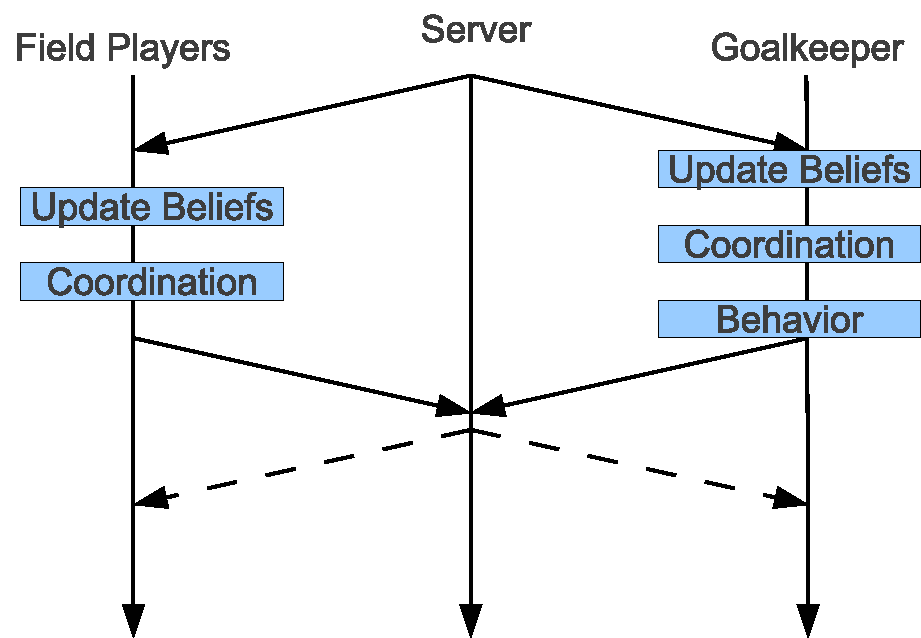
\includegraphics[width=0.6\textwidth]{Chapter4/figures/CoordinationCycle.pdf}
  \caption{The Coordination Protocol.} 
  \label{fig:CoordinationCycle}
\end{figure}


Figure~\ref{fig:CoordinationCycle} shows the entire coordination protocol (which may last several simulation cycles). All players initially update their beliefs. The coordinator (goalkeeper) waits for messages from all other players. Once these messages are gathered at the coordinator, the coordination procedure is executed and the resulting actions for each player are communicated back to the players. At this point all players execute their actions, in essence realizing their behavior. We selected the goalkeeper to act as coordinator, because its role is quite distinct and independent from the other players and therefore it can afford to dedicate more computational resources to the team coordination algorithm compared to the other players. 

The team coordination procedure executed only by the coordinator after all messages have been received is split in several phases:
\begin{description}
%\item[Gather Coordination Messages] The coordinator waits for all players to submit their local beliefs about the world state. This phase is completed as soon as all messages have been received. 
\item[Update Coordination Beliefs] The local world state beliefs from the other players are combined in order to update the global belief about the world state (global ball location, distances of all players from the global ball location, locations of all players). 
\item[Determine Coordination Subsets] Field players are split into non-overlapping subsets according to their significance in the current game state. These subsets are:
\begin{itemize}
\item \textit{Goalkeeper}: one player, the goalkeeper
\item \textit{Inactive}: players fallen on the ground or players with lost self-location
\item \textit{Active}: three players, the ones closest to the ball
\item \textit{Support}: all remaining players
\end{itemize}
\item[Determine Active Positions] Several candidate positions are determined for the active players.
\item[Coordinate Active Players] The active player closest to the ball is assigned to go to the ball and the best pair of candidate positions is selected for the remaining active players according to a cost function.
\item[Generate Team Formation] A formation is generated for the entire team (excluding the goalkeeper) depending on the current position of the ball in the soccer field.
\item[Assign Team Roles] All team players, except the goalkeeper, are assigned roles taking into account the desired  formation of the team and their current position.
\item[Determine Support Positions]  Candidate positions are determined for the support players. These are determined by the desired team formation, after excluding the roles assumed by the active players and a number of least-significant roles equal to the number of inactive players. 
\item[Coordinate Support Players] The best mapping between support players and support positions according to a cost function is computed.
\end{description}
Algorithm~\ref{CoordinationAlgorithm} describes the entire coordination procedure, which currently lasts six simulation cycles. In each simulation cycle, some, but not all, of the above phases are executed. This choice was dictated by the time limitation of the agent think cycle; with this choice, each group of phases fits within a single simulation cycle causing no delays and enabling real-time operation. 

\begin{algorithm}[ht!]
\caption{Coordination Protocol }
\label{CoordinationAlgorithm}
\begin{algorithmic}[1]
\begin{small}
\STATE {\bf Input: }$Coordination Messages = \lbrace M_{1},M_{2},...,M_{N-1} \rbrace, N = Number Of Players $
\STATE {\bf Output: }$Actions = \lbrace A_{1},A_{2},...,A_{N-1} \rbrace$
\STATE
\IF {$ CoordinationCycle = 1$ }
\STATE $B \leftarrow Update Coordination Beliefs(Coordination Messages) $
\STATE $CoordinationCycle = CoordinationCycle + 1$
\ELSIF {$ CoordinationCycle = 2$ }
\STATE $S \leftarrow Determine Coordination Subsets(B) $
\STATE $CoordinationCycle = CoordinationCycle + 1$
\ELSIF {$ CoordinationCycle = 3$ } 
\STATE $P_{active} \leftarrow Determine Active Positions(B,S) $
\STATE $CoordinationCycle = CoordinationCycle + 1$
\ELSIF {$ CoordinationCycle = 4$ }
\STATE $A_{active} \leftarrow Coordinate Active Players(P_{active},S,B) $
\STATE $CoordinationCycle = CoordinationCycle + 1$
\ELSIF {$ CoordinationCycle = 5$ }
\STATE $ F \leftarrow Generate Team Formation(B) $
\STATE $ R \leftarrow Assign Team Roles(A_{active},B,F) $
\STATE $ P_{support} \leftarrow Determine Support Positions(R,F,S) $
\STATE $CoordinationCycle = CoordinationCycle + 1$
\ELSIF {$ CoordinationCycle = 6$ }
\STATE $A_{support} \leftarrow Coordinate Support Players(P_{support},S,B,R,F,A_{active}) $
\STATE $Actions = A_{active} \cup A_{support} \cup A_{inactive}$
\STATE $CoordinationCycle = 0$
\ENDIF
\end{small}
\end{algorithmic}
\end{algorithm}


\section{Coordination Modes}

Coordination is not a static procedure and may change dynamically during different game states. There are three modes of team coordination:
\begin{description}
\item[Active] This is the normal mode of coordination. Every aspect of the coordination process we have discussed above is used for the team's coordination and the computation of action for all field players.
\item[Support] In this mode, all players, excluding the goalkeeper, join by default the support subset. It is used in situations where our goalkeeper takes control of the ball or where only the opponent team has the right to perform a kick to the ball, e.g. opponent's kick-off,  opponent's goal kick, etc.
\item[Wait] In this mode, all players, excluding the goalkeeper, join by default the inactive subset. It is used in situations where both teams have to wait for the kick-off signal before a kick-off.
\end{description}


\section{Coordination and Communication}
Coordination is accomplished through communication. We use the common communication channel through the simulation server in order to provide the messaging between players involved in the coordination process. For this reason, communication plays a major role in our approach. The general idea of this communication process among players is that the coordinator (goalkeeper) needs to know all agents' beliefs about the world state before proceed with the execution of the coordination protocol. Furthermore, communication is needed to send the outcome of coordination from the coordinator to all players. 

There are several types of messages, each one of them having different functionality and serving a specific purpose. The arguments of each message are preceded by a single-letter identifier indicating the type of the message. The message types used in our coordination protocol are:
\begin{description}
\item[Init Message] This type of message declares the presence of each agent in the simulation environment. All players, other than the coordinator, must send this message to the coordinator before the coordination protocol begins.
\begin{description}
  \item[{\bf Message format:}] 
  \texttt{i,<Agent Uniform Number> }
\end{description}

\item[Start Message] This type of message is sent only by the coordinator; it declares that all agents are now initialized and ready to begin the coordination process. Each agent receiving this message should immediately start sending coordination messages.

\begin{description}
  \item[{\bf Message format:}] 
  \texttt{s,<Coordinator Uniform Number>}
\end{description}

\item[Coordination Message] This is the most important type of message. It includes information about each agent's beliefs. There are four subtypes of this message depending on  the current beliefs of the agent:
\begin{description}

\item[Type C] The agent has complete awareness of the ball and self location; the message includes the uniform number, the self position, and the ball position.

\begin{description}
  \item[{\bf Message format:}]
  \texttt{c,<Agent Uniform Number>,<Agent X>,<Agent Y>,\\<Ball X>,<Ball Y>}
\end{description}

\item[Type L] The agent has complete awareness only of his own position in the field; the ball is not currently within the field of view and, even though there may be a filtered belief about the ball location, it is better to avoid sending possibly faulty information. The message includes only the uniform number and the self position.

\begin{description}
  \item[{\bf Message format:}]
  \texttt{l,<Agent Uniform Number>,<Agent X>,<Agent Y>}
\end{description}

\item[Type B] The agent has complete awareness of the ball's location, only with respect to itself. The message includes the uniform number, the distance of the ball and the horizontal angle of the ball relative to its own body angle.

\begin{description}
  \item[{\bf Message format:}]
\texttt{b,<Agent Uniform Number>,<Ball Distance>,<Ball Angle>}
\end{description}

\item[Type X] The agent has complete unawareness of the ball and self location or has fallen on the ground. The message includes only the uniform number. These agents join the inactive subset.

\begin{description}
 \item[{\bf Message format:}]
 \texttt{x,<Agent Uniform Number>}
\end{description}

\end{description}
\item[End Message]
This type of message asks the players, other than the coordinator, to stop sending coordination messages. At this point, the coordinator is ready to execute the coordination procedure and calculate actions for all players.
\begin{description}
  \item[{\bf Message format:}] 
  \texttt{e,<Coordinator Uniform Number>}
\end{description}
\item[Action Message]
This type of message is sent only by the administrator; it declares which action each agent has been assigned by the coordination process. These messages are sent at the end of the coordination procedure, when actions for all players have been computed. The message includes the uniform number of the recipient agent, the action identifier, and the possible action parameters. 
\begin{description}
  \item[{\bf Message format:}]
  \texttt{a,<Agent Uniform Number>,<Action ID>,<Action Parameters>}
\end{description}

\end{description}

\begin{figure}[t!]
\centering
  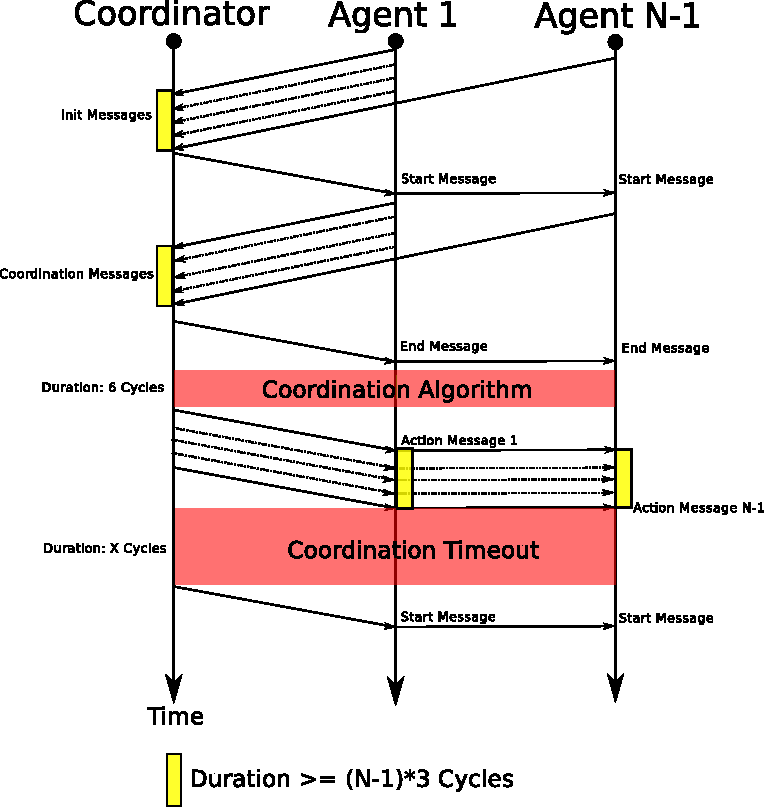
\includegraphics[width=0.8\textwidth]{Chapter4/figures/CoordComm.pdf}
  \caption{Communication Process in Coordination.} 
  \label{fig:coordinationprocess}
\end{figure}

Figure~\ref{fig:coordinationprocess} presents the messaging procedure between the agents in order to coordinate their actions. First, agents have to initialize their presence in the field with ``init'' messages. The coordinator saves these messages and, when all other players have initialized themselves, broadcasts a ``start'' message. This message means that all players are now ready to start the coordination process. In this phase, all players, other than the coordinator, send their ``coordination'' messages to the coordinator. When the coordinator gathers these messages from all players, it broadcasts an ``end'' message to make them stop sending unnecessary ``coordination'' messages. The next phase of this process is the execution of the coordination protocol which lasts six simulation cycles, approximately 120ms. When it finishes, the coordinator broadcasts the resulting actions to each one of the other players using individual ``action'' messages. The receiving agents execute the commanded actions, until a new ``action'' message arrives. While action execution is ongoing, after a timeout period defined by the user (currently set at 20 simulation cycles), the same coordination process is repeated, excluding the initialization phase.


\section{Coordination Beliefs Update}
\label{sec:UpdateBeliefs}

In the previous section we presented how players exchange messages with the coordinator. In this section we are going to discuss how the coordinator fuses the individual beliefs received by the other agents into a single global belief. This step is of major importance in any multi-agent system. Having multiple observations of the same world could potentially be a problem. The coordinator has to combine these observations without knowing which one of them is faulty or correct in order to obtain a global realistic representation of the world. Knowledge of the ball and agents' positions is sufficient to execute the coordination algorithm without making guesses.

The global ball position is computed taking into account only the information communicated by the agents using ``type C'' coordination messages. Furthermore, information of the coordinator is taken into account, if the coordinator also has sufficient knowledge about the ball and self location. Apparently, the maximum number of ball observations at any time is the number of all agents, when all of them have sufficient knowledge about the ball and self location.
\begin{figure}[t!]
\centering
  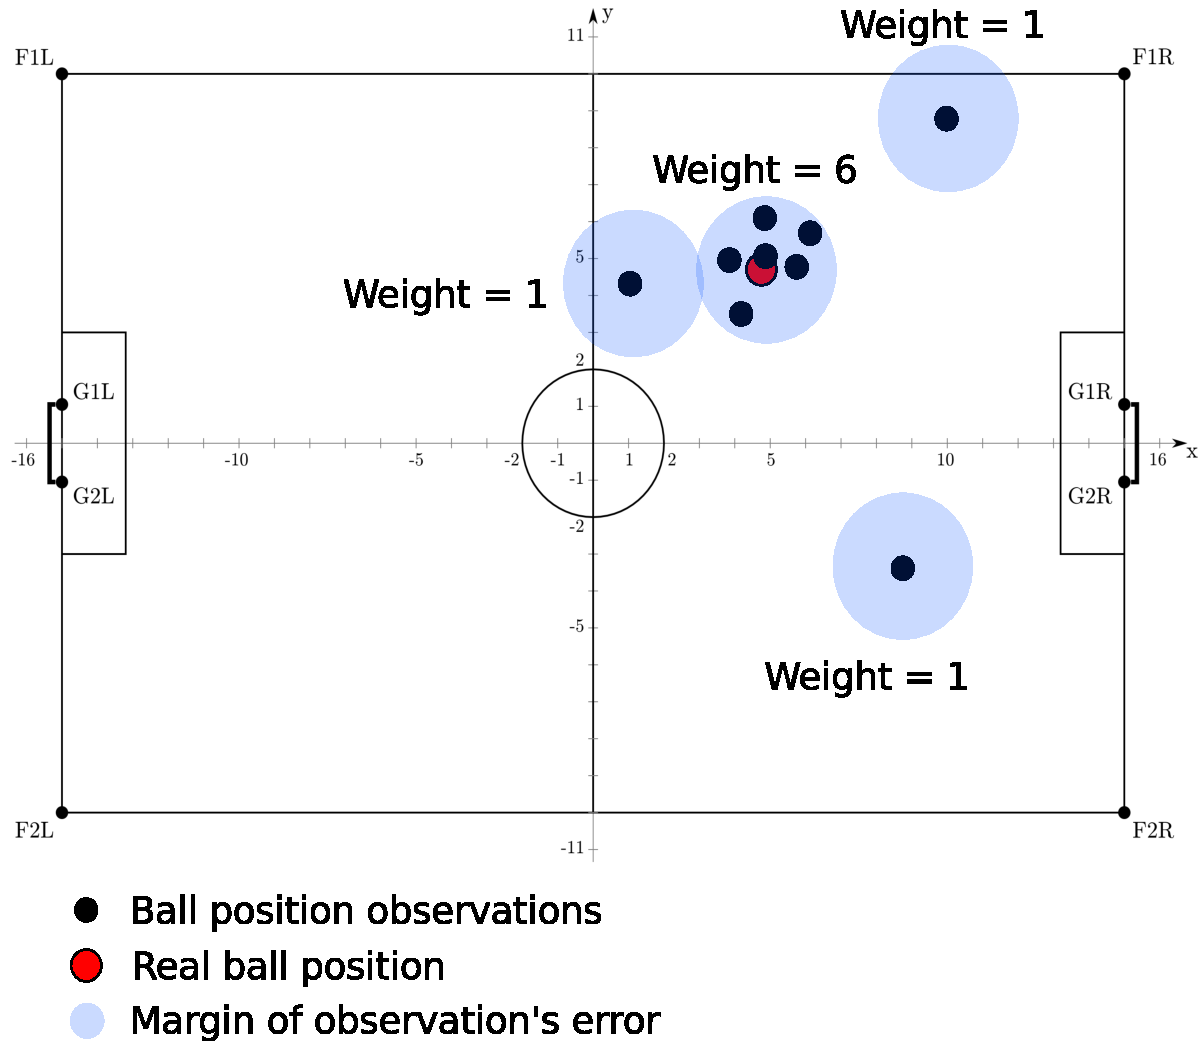
\includegraphics[width=0.8\textwidth]{Chapter4/figures/Ball.pdf}
  \caption{Global Ball Position Estimation from Multiple Ball Observations.} 
  \label{fig:Ball}
\end{figure}
As shown in Figure~\ref{fig:Ball}, different ball observations can differ from each other. In our approach, we use a simple algorithm to estimate the global ball position with accuracy. A threshold is defined (by default, 1 meter) in order to split the observations in clusters. %Each cluster is assigned a weight equal to the number of observations it contains. Additionally, 
Each cluster is represented by the average of the observations it contains. The first incoming observation defines the first cluster. For each subsequent incoming observation, we check its distance against all representatives of all existing clusters. Focusing only on the distances that fall below the threshold and the corresponding cluster, the new observation is assigned to the largest of these clusters, updating at the same time the representative of that cluster. Otherwise, the new observation gives rise to a new cluster with a single member. Each cluster is assigned a weight so that the cluster with the most observations is naturally assigned the biggest weight. Our choice for the weight function is the size $|s_i|$ of cluster $s_i$ cubed, that is $w(s_i) = |s_i|^3$.
Figure~\ref{fig:Ball} shows the resulting four cluster for a given set of nine observations.  Consequently, we have to compute our belief about the global ball position. This is taken to be the weighted average of the cluster representatives. More specifically, given $m$ clusters $s_i$ containing ball observations $o_{ij}$ each, the final ball belief is computed as:
\begin{align*}
{\bf Global Ball Belief} = \sum_{i=1}^m \frac {w(s_i)} {\sum_{k=1}^m w(s_k)} \sum_{o_{ij} \in s_i} \cfrac{o_{ij}}{|s_i|}
\end{align*}


The next step towards forming the global belief is to determine each agent's position and its distance from the estimated global ball position. Players who have sent a ``Type C'' or ``Type L'' coordination message have already communicated their exact position in the field; their distance from the ball is simply calculated as the distance between the estimated global ball position and the players' position. Players who have sent a ``Type B'' coordination message don't know their exact position in the field, but this can be inferred using the estimated global ball position and the information they submitted about the distance and angle of the ball observation with respect to themselves; their distance from the ball is simply the one they reported. Finally, for players who have sent a ``Type X'' coordination message, we assume an infinite distance to distinguish them from all other players; their position in the field cannot be inferred. 


\section{Determination of Coordination Subsets}
The existence of multiple agents makes coordination a complex and computationally expensive problem to be solved by a single agent. In our case, the coordinator (goalkeeper) would have to solve this huge problem for a total of nine players or eleven players (depending on the server's version).
Instead of trying to solve the coordination problem at one level, a simple approach is to first decompose the problem into smaller coordination problems and then solve each one of them in isolation. To this end, we split the players into small subsets in which coordination can be achieved quickly to meet real-time requirements. In our approach, there are four such subsets:

\begin{description}
\item[Goalkeeper] This subset includes only one agent, the goalkeeper. The player with the uniform number $1$ is selected to be the agent responsible for guarding our goal. Goalkeeper also serves as the coordinator. His independent and individual behavior is explained in Section~\ref{GoalKeeper}.

\item[Inactive subset] The Inactive subset consists of agents who have sent ``Type X'' coordination messages, that is players fallen on the ground or players with lost self-location. It is the less important subset of agents in the coordination procedure and in fact there is no need to coordinate them. Agents in this subset are assigned the same action, namely the Turn to Localize action. After they find their positions, they will have a chance to enter the active or support subsets in the next coordination cycle.

\item[Active subset] The Active subset consists of three agents, the ones closest to the ball, and it is the most important subset of agents in the coordination. Agents in this subset are responsible for executing the most critical actions for their team. Moreover, due to the small size of this subset, we can afford to solve their coordination problem by exhaustive enumeration to obtain an optimal solution. 

\item[Support subset] The Support subset consists of all remaining agents. The size of this subset, which varies between 0 and 8 or 10 (depending on the server's version), may result in prohibitive computational costs for optimal coordination, therefore we adopt an approximate, yet effective, coordination method based on dynamic programming.
\end{description}
Figure~\ref{fig:Splitter} presents an example of coordination subsets. Assuming that all agents have complete awareness of their position, it is easy to realize that the agents within the red distance threshold will join the active subset and the other five agents who have farther distances from ball (yellow distance threshold) will join the support subset. Moreover, a possible existence of one or more agents having unawareness about the world state, should lead them joining the inactive subset. The goalkeeper is in its own subset. 

\begin{figure}[t!]
\centering
  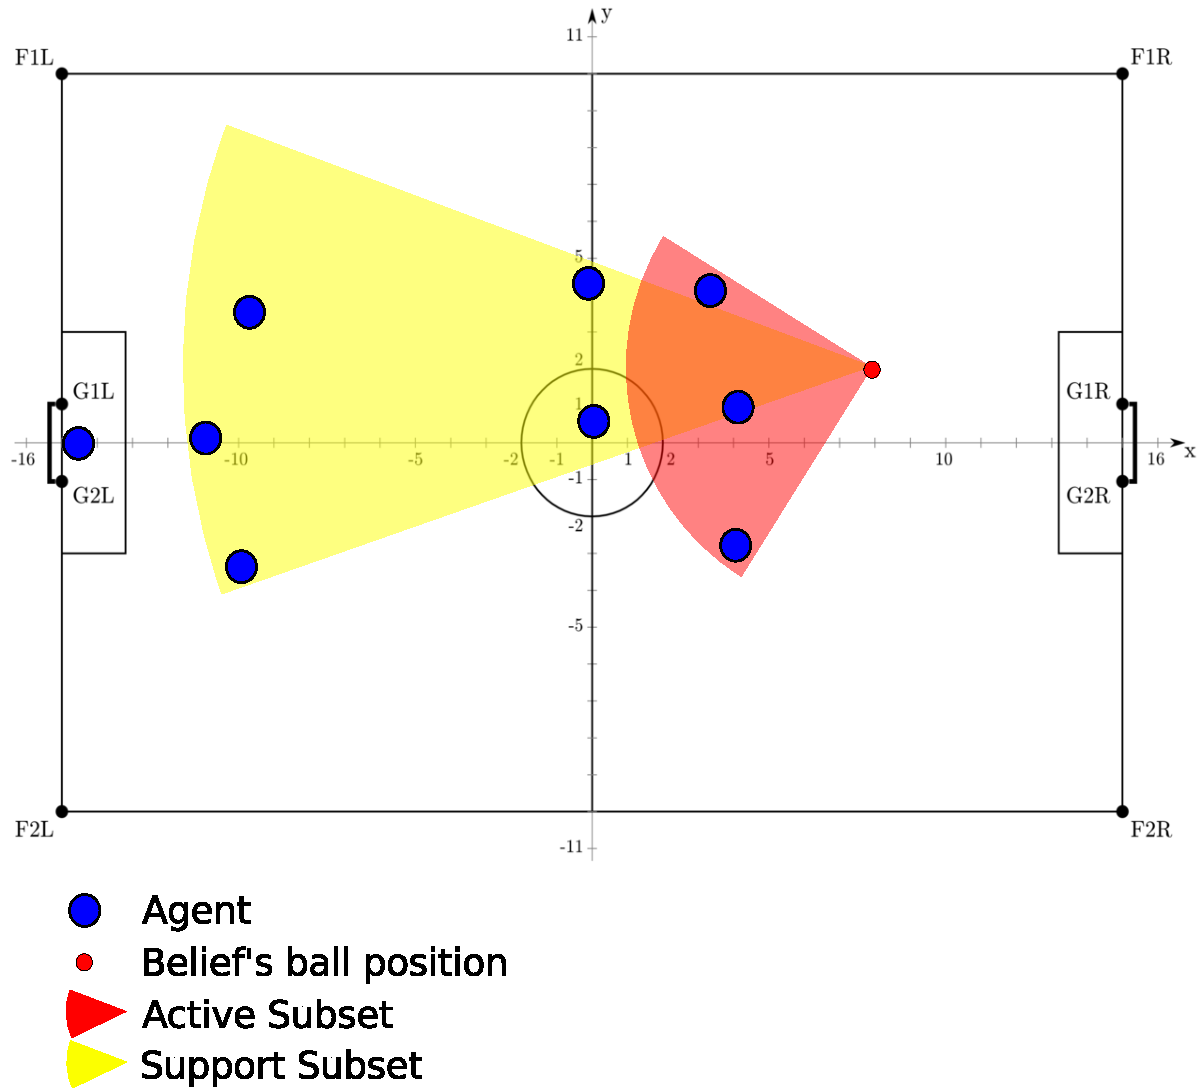
\includegraphics[width=0.8\textwidth]{Chapter4/figures/Splitter.pdf}
  \caption{Coordination Splitter.} 
  \label{fig:Splitter}
\end{figure}



\begin{figure}[t!]
\centering
  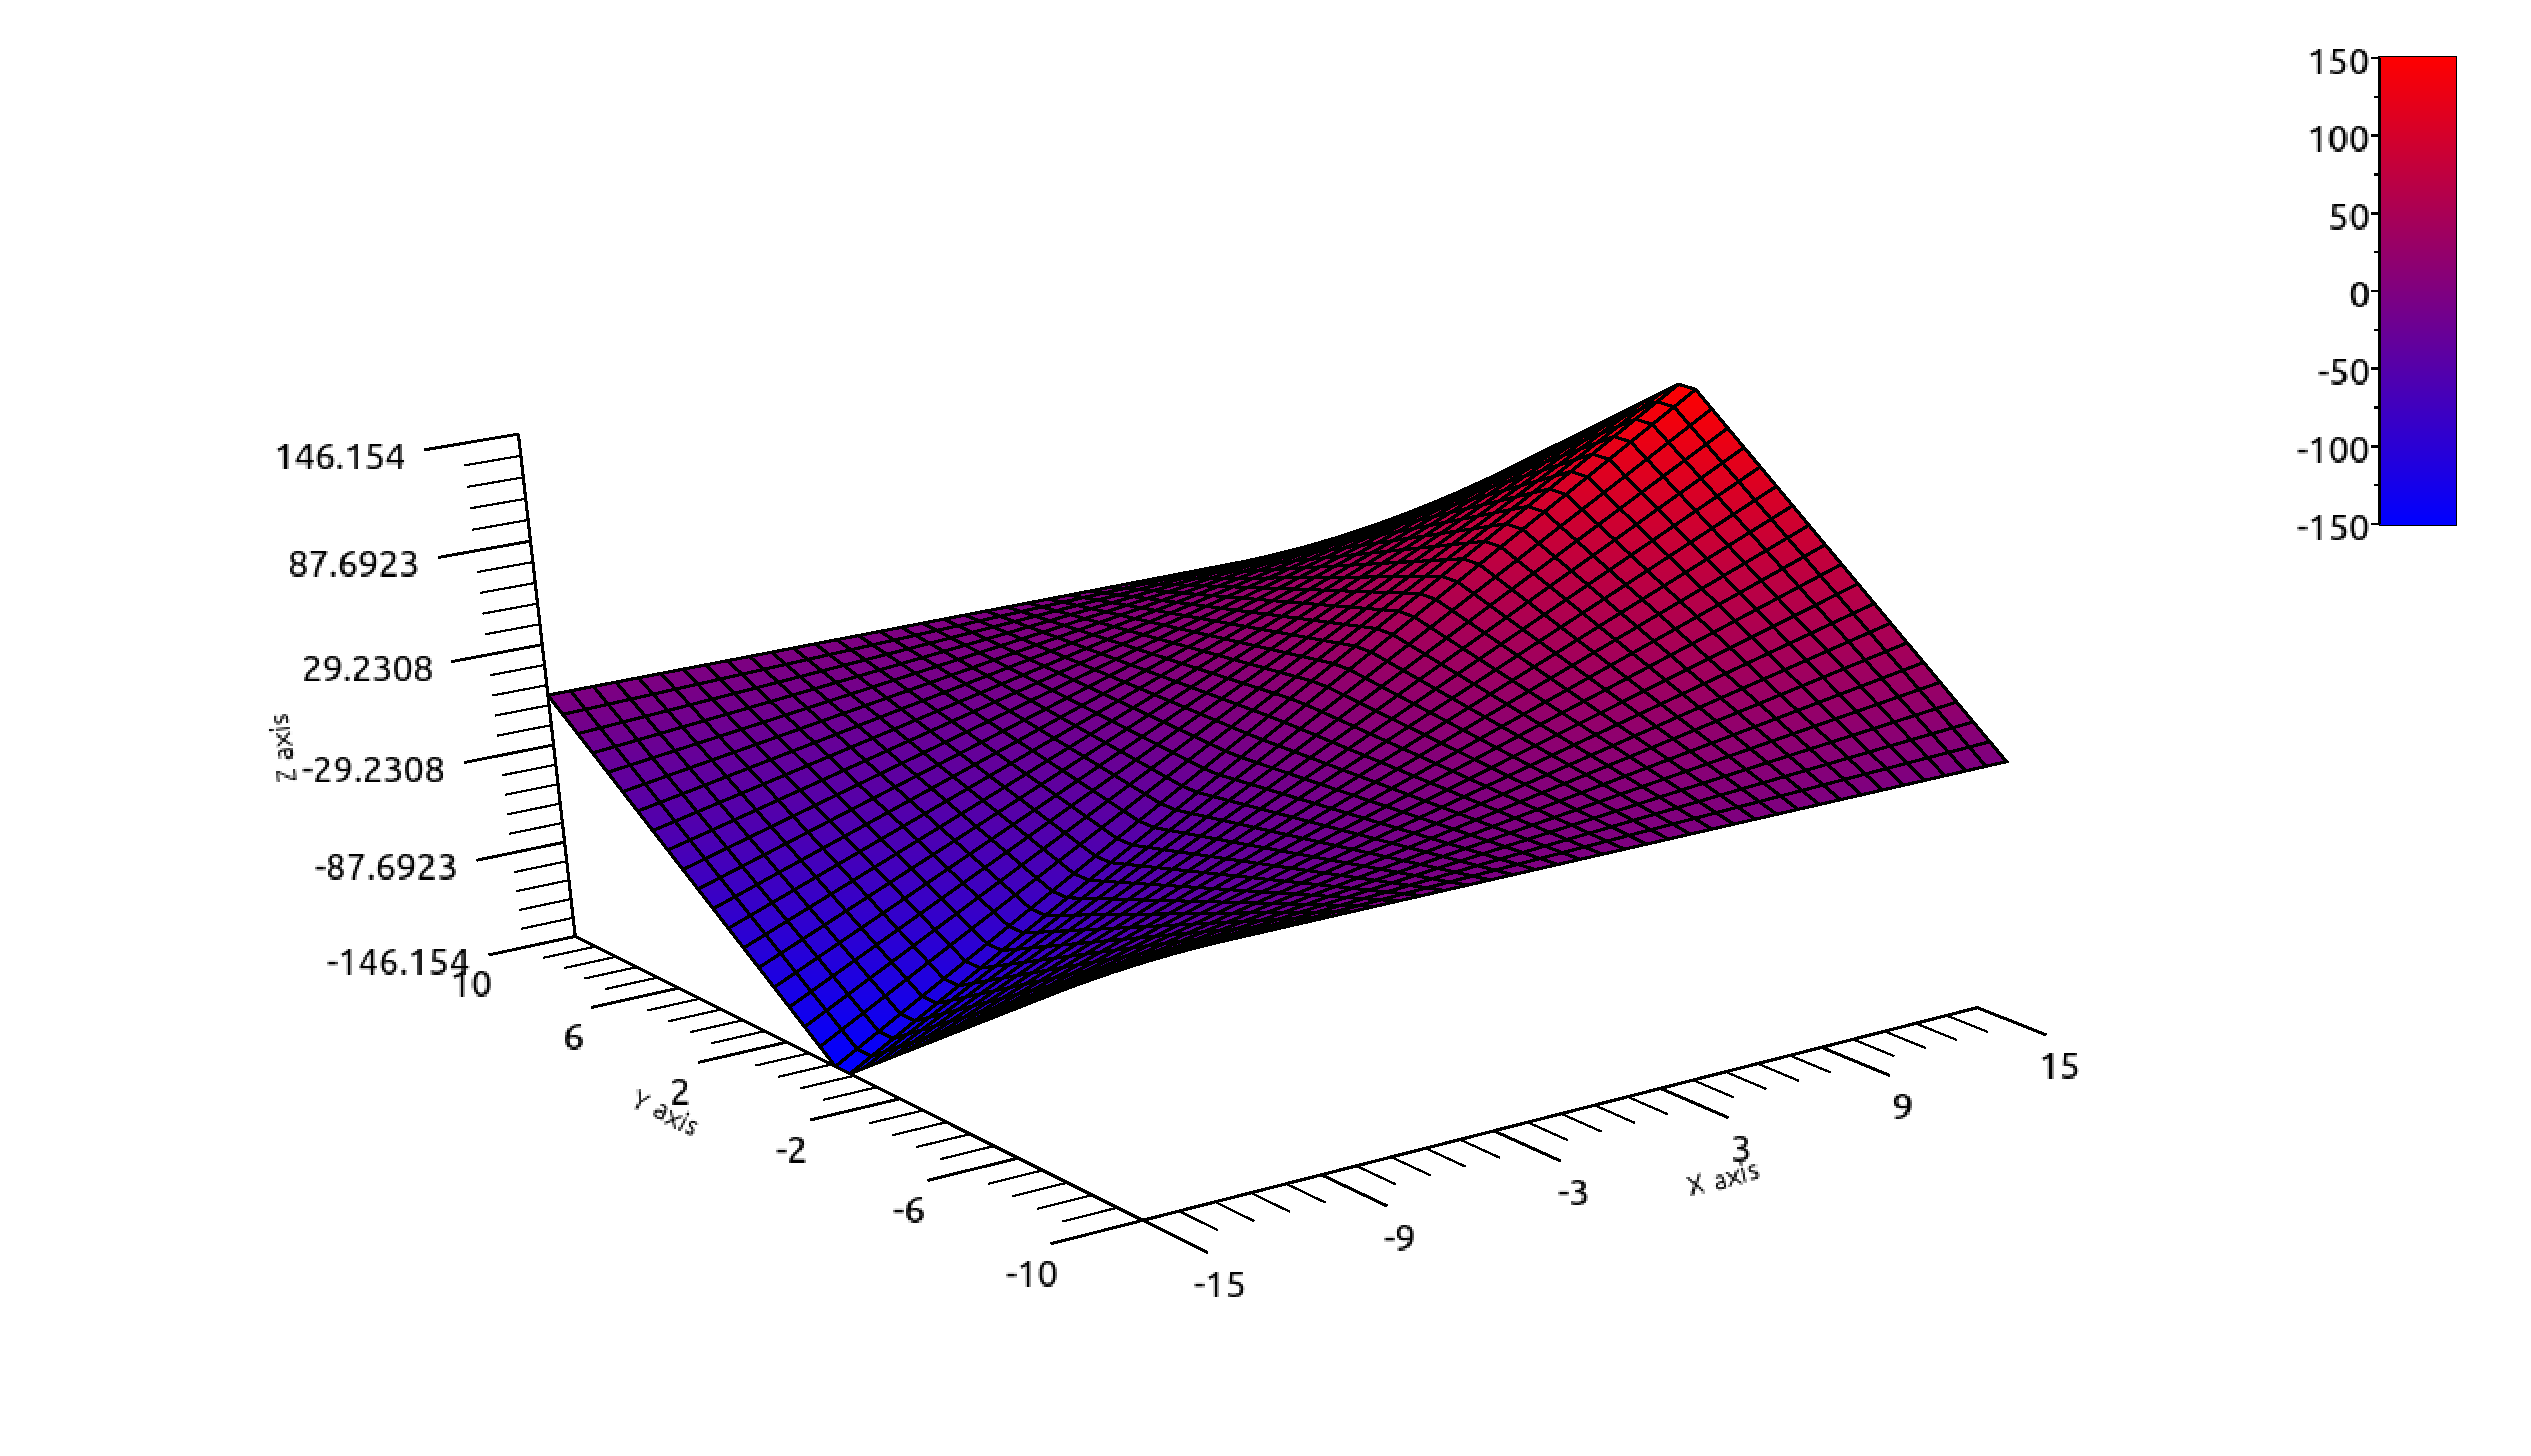
\includegraphics[width=\textwidth]{Chapter4/figures/Graph1.pdf}
  \caption{Soccer Field Value.} 
  \label{fig:SoccerValue}
\end{figure}



\section{Soccer Field Utility Fuction}
\label{FieldValue}

In order to proceed our discussion about the coordination process, we have to define a simple, yet functional, way to give a value to every spot of the soccer field. Figure~\ref{fig:SoccerValue} presents this utility function over the entire soccer field, whose analytical form is: 
\[
FieldUtility(x,y) = CurrentSide \times x \times \left(\cfrac{FieldWidth}{2} - |y|\right) 
\]
where $CurrentSide$ is either $+1$ or $-1$ depending on the side of the field we currently play, so that the highest value corresponds to the opponent's goal. 
The key idea is that, as the ball is heading towards the opponent goal, this value is becoming higher. In contrast, as the ball is heading towards our goal, this value is becoming lower. It is easy to realize that a high value at some spot means more chances to score a goal, whereas a spot with small value implies a dangerous game situation. This function will prove to be useful in the next steps of the coordination process.




\section{Determination of Active Positions}
Until now, we have updated the coordination beliefs and we have split agents into subsets. In this phase of the coordination process, we have to compute promising candidate positions for the Active subset. We distinguish between two cases. In the first case, the ball is located in our half of the field. In this case we have to find candidate positions which have a defensive approach. In the other case, if the ball is located in the opponent's half of the field, we have to find candidate positions which have an offensive approach. 

In both cases, we start by creating a set of equidistant positions around the ball located at different radii, discarding any such positions that fall outside or near the soccer field's limits. For the defensive approach, we choose 12 positions at a radius of 1 meter and $30^\circ$ apart and another 12 positions at a radius of 1.5 meters and $30^\circ$ apart. For the offensive approach, we choose 12 positions at a radius of 2 meters and $30^\circ$ apart and another 24 positions at a radius of $\max\{3,(|x|+|y|)/(FieldLength/2+FieldWidth/2)\}$ meters and $15^\circ$ apart. The idea in the offensive case, is that the more we approach the corners of the field, the more the candidate positions are spread around the ball. Figure~\ref{fig:ActivePositions2} shows how these positions are determined in two different scenarios. 



These sets of candidate positions is further filtered using the soccer field utility function. In the defensive case, we keep up to nine positions, the ones with the least utility values. These positions will mostly be between the ball and our own goal aiming to protect against an opponent strike. In the offensive case, we keep up to nine positions, the ones with the highest utility values. These positions will mostly be between the ball and the opponent's goal aiming to position players at attacking spots. Figure~\ref{fig:ActivePositions3} shows the filtered sets of candidate positions for the Active subset in the same scenarios.

\begin{figure}[t!]
\centering
  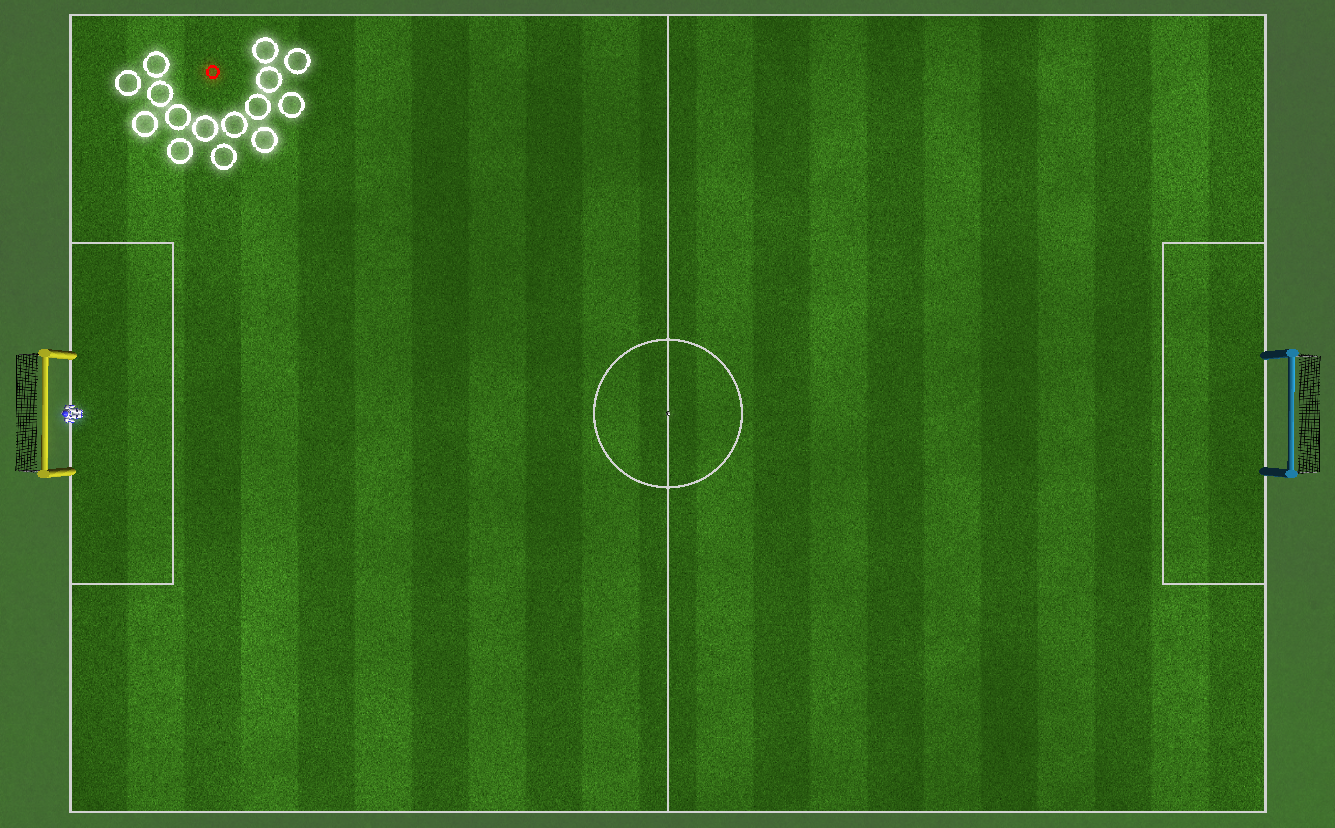
\includegraphics[height=5cm, clip, trim=0cm 10cm 20cm 0cm]{Chapter4/figures/ActiveBefore(-8,6).png} \	
  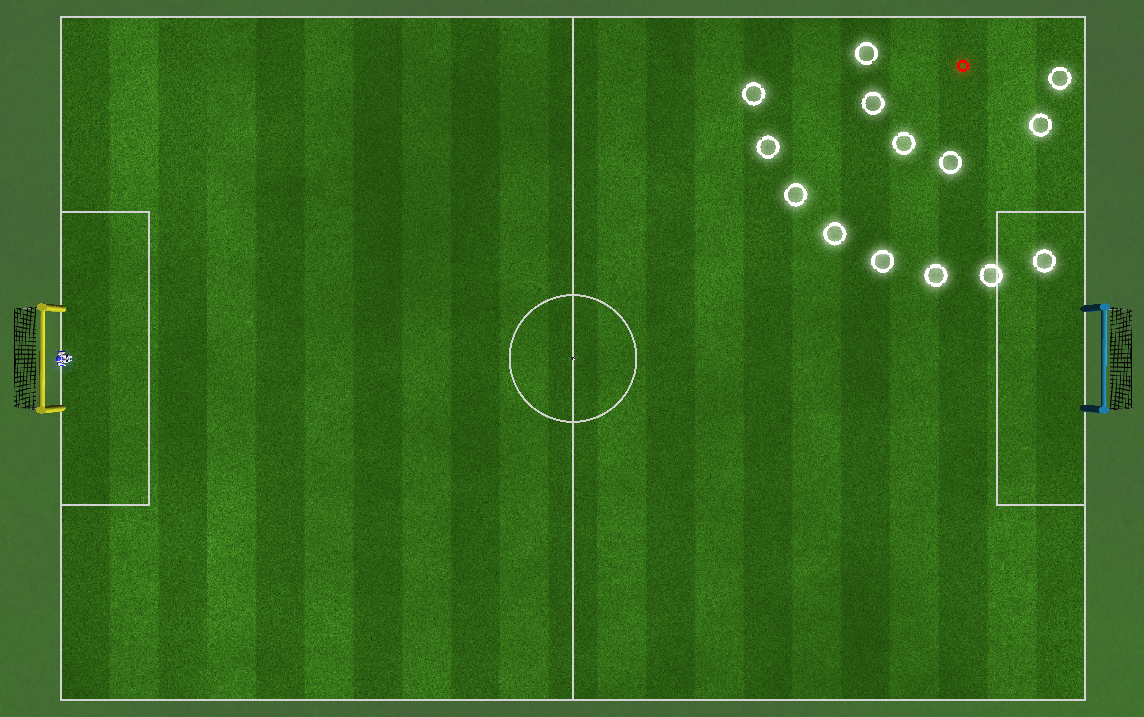
\includegraphics[height=5cm, clip, trim=20cm 10cm 0cm 0cm]{Chapter4/figures/ActiveBefore(8,6).png}
  \caption{Initial Candidate Active Positions: Defense (left) and Offense (right).} 
  \label{fig:ActivePositions2}
\end{figure}

\begin{figure}[t!]
\centering
  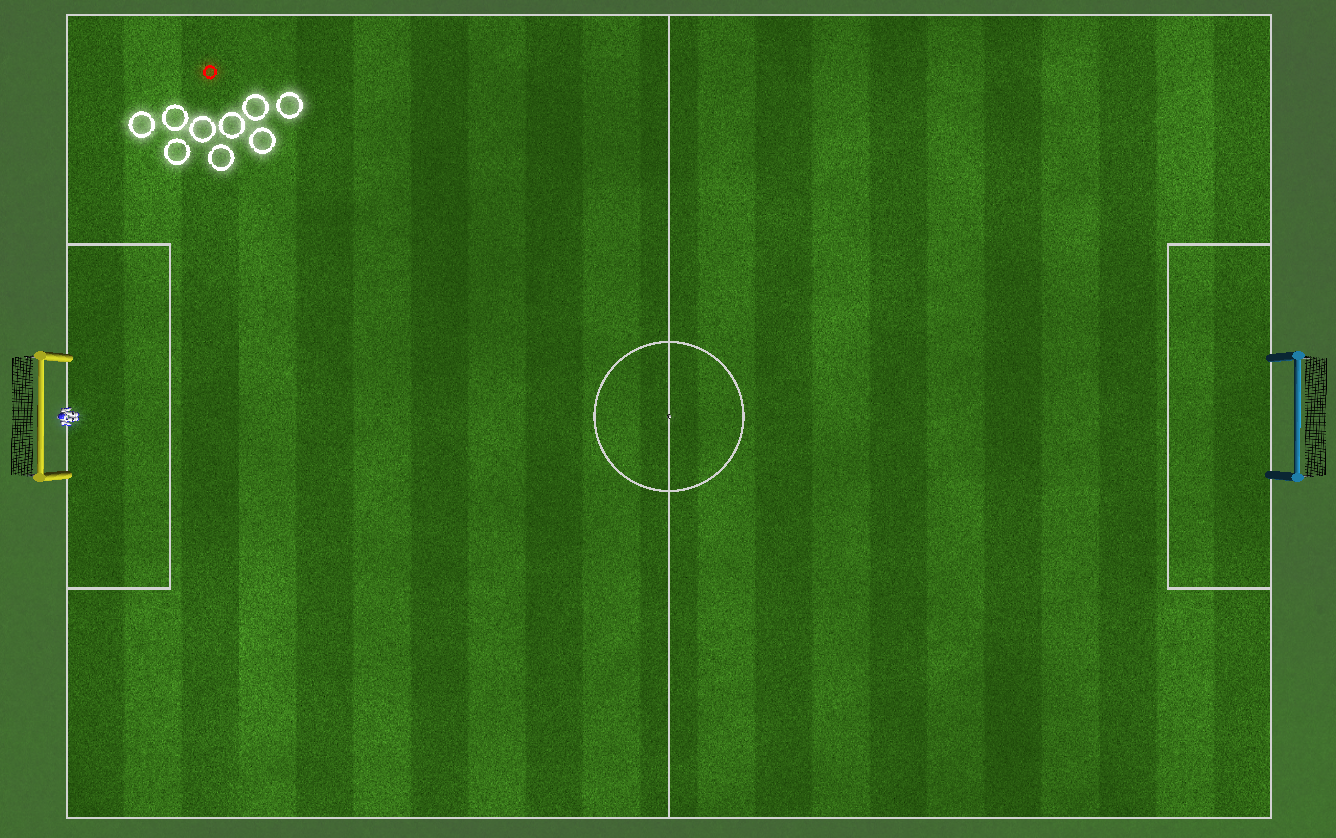
\includegraphics[height=5cm, clip, trim=0cm 10cm 20cm 0cm]{Chapter4/figures/ActiveAfter(-8,6).png} \	
  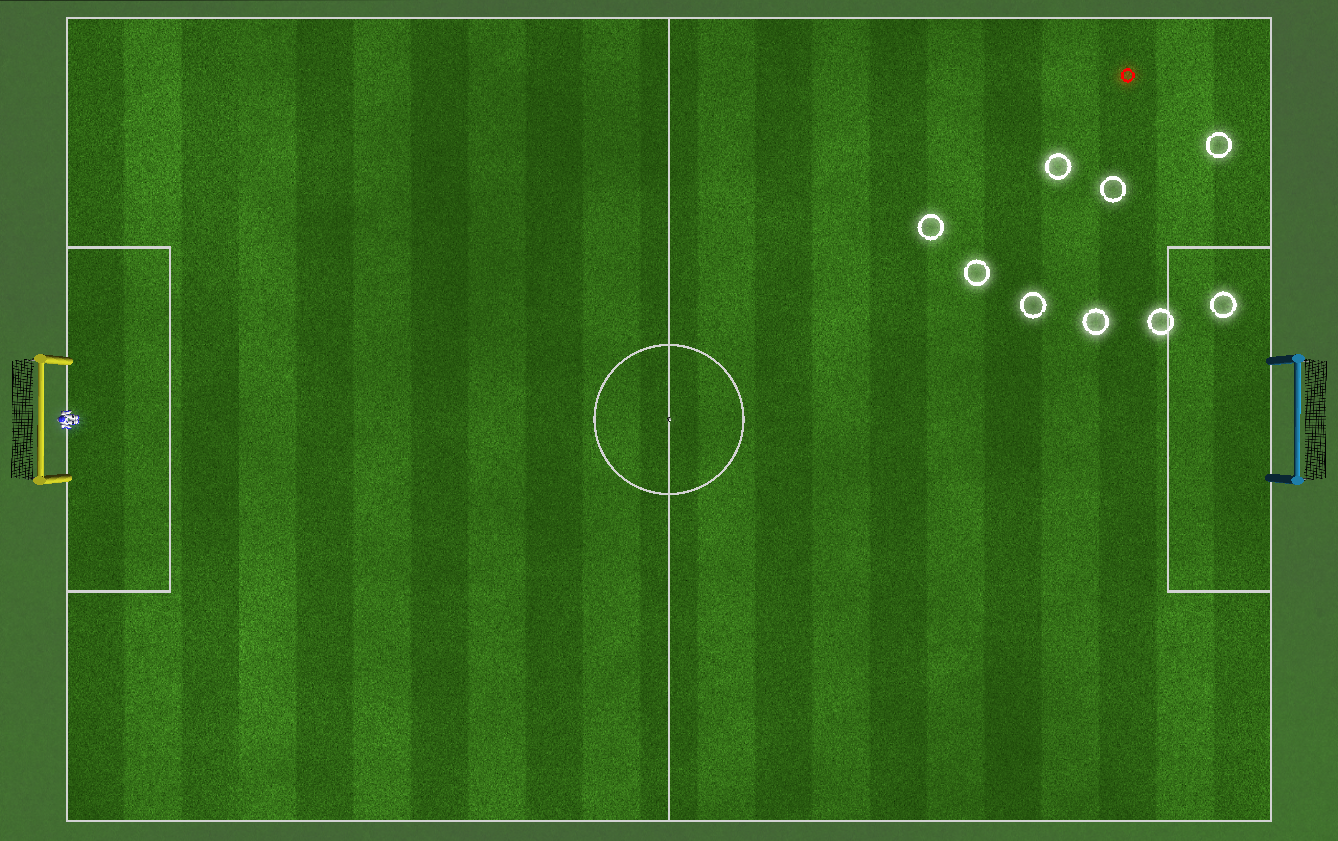
\includegraphics[height=5cm, clip, trim=20cm 10cm 0cm 0cm]{Chapter4/figures/ActiveAfter(8,6).png}
  \caption{Final Candidate Active Positions: Defense (left) and Offense (right).} 
  \label{fig:ActivePositions3}
\end{figure}


\section{Active Players Coordination}
\label{sec:ActiveCoordination}
Our coordination scheme for the Active subset requires that one player will undertake the task of approaching the ball, whereas the other two players will have to choose a pair of positions from the candidate Active positions.  This is accomplished by a mapping function.  

\subsubsection*{Player on Ball}
An agent from the Active subset has to be selected in order to execute the On Ball action. We have to find the agent who minimizes a weighted sum over the following two terms:
\begin{enumerate}
\item \textbf{Distance from ball} $d_{i}$, the distance of agent $i$ from the ball. 
\item \textbf{Angle towards goal} $\vartheta_{i}$, the sum of the absolute angles between the agent and the ball and between the ball and the opponent's goal.
\end{enumerate}
Given an Active subset with 3 players, the On Ball player is determined as follows:
\begin{align*}
{\bf ActiveSubset} &= \lbrace Agent_{1},Agent_{2},Agent_{3} \rbrace  \\
{\bf Value_{i}} &= d_{i} + a \vartheta_{i}, \text{where $a\in\mathbb{R}$ is a weight, default=$0.01$} \\
{\bf OnBallPlayer} &= \arg\min_{i}(Value_{i})
\end{align*}
Additionally, we give a small advantage to the agent who had been assigned this action in the previous coordination cycle over the other players. We do this to prevent continuous changes in the assignment of the On Ball player, when several two agents have similar distances and angles from the ball. This advantage takes the form of a value decrease (default: 1).


\begin{algorithm}[t!]
\caption{Active Players Optimal Mapping}
\label{ActiveMapping}
\begin{algorithmic}[1]
\STATE {\bf Input: }$ActivePlayers = ActiveSubset - OnBallPlayer = \{Agent_1,Agent_2\}$
\STATE {\bf Input: }$ActivePositions = \lbrace P_{1},P_{2},...,P_{N} \rbrace, N\leq 9 $
\STATE {\bf Output: } $Optimal Active Mapping$
\STATE 
\STATE $OptimalActiveMappingCost = +\infty$
\FOR{{\bf each} $(P_i,P_j) \in ActivePositions \times ActivePositions, i\neq j$}
\STATE $ActiveMapping = \{Agent_1 \leftarrow P_i,\ Agent_2 \leftarrow P_j,\ OnBallPlayer \leftarrow Ball\}$
\STATE $ActiveMappingCost = ActiveCost(ActiveMapping)$
\IF{$ActiveMappingCost < OptimalActiveMappingCost$}
\STATE $OptimalActiveMapping = ActiveMapping$
\STATE $OptimalActiveMappingCost = ActiveMappingCost$
\ENDIF
\ENDFOR
\RETURN $OptimalActiveMapping$
\end{algorithmic}
\end{algorithm}




\subsubsection*{Active Players Optimal Mapping}
Next in the active coordination phase, we have to assign positions for the other two agents  left in the Active subset. Algorithm~\ref{ActiveMapping} shows how we can find the optimal mapping by exhaustively enumerating and evaluating each possible assignment. During evaluation, we also take into account the position assignment of the On Ball agent, which will be helpful in order to find possible collisions between the On Ball agent and the remaining active ones. More specifically, the evaluation function scores each possible mapping using the following features defined for each agent $i$: 

\begin{enumerate}
\item \textbf{Distance} $C_{d,i}$ - This is the distance between the current and the target positions of agent $i$. Agents try to minimize this feature to be able to reach their target positions as soon as possible. 
\item \textbf{Potential Collisions} $C_{c,i}$ - Approximating the route of each agent as a straight line between the current and the target positions, we check if the route of agent $i$ intersects with the routes of the other two agents. For any pair of routes, if there is no intersection, the cost is 0 (infinitesimal probability of collision). If there is intersection and the intersection point is approximately equidistant from the current positions (the absolute difference is less than 1.5 meters), the cost is 100 (high probability of collision). Finally, if there is intersection but the intersection point is not equidistant from the current positions, the cost is 2 (small probability of collision). This feature returns the sum of these costs over the two pairs of routes considered for agent $i$. Figure~\ref{fig:AvoidCollision} shows the key idea behind the detection of a possible collision between two agents. If $|d_{1}-d_{2}|\le 1.5$, a collision is highly possible. Agents try to minimize this feature to avoid collisions.
\item \textbf{Field Utility} $C_{u,i}$ - This is the absolute value of the field utility (cf. Section~\ref{FieldValue}) for the position assigned to player $i$. Agents try to maximize this feature to give preference to positions with better utilities.
\item \textbf{Close Targets} $C_{t,i}$ - This is the sum of absolute differences between the target positions of agent $i$ and the other two agents. Agents try to maximize this feature to give preferences to targets that are not too close.
\item \textbf{Horizontal Stretch} $C_{h,i}$ - This is the sum of absolute differences between the $X$-axis coordinates of the target positions of agent $i$ and the other two agents. Agents seek to maximize this feature to stretch horizontally in the field and have better region coverage and unblocked fields of view.  
\end{enumerate}
The features described above are computed for each of the three agent, are weighted, and are summed to form the final evaluation function of a mapping: 
\begin{align*}
ActiveCost(ActiveMapping) &= \sum_{i=1}^3 w_dC_{d,i}+w_cC_{c,i}-w_uC_{u,i}-w_tC_{t,i}-w_hC_{h,i}
\end{align*}
where $(w_d,w_c,w_u,w_t,w_h)$ are the weights of the features, currently set at $(1,1,1/7,1,1)$.

\begin{figure}[t!]
\centering
  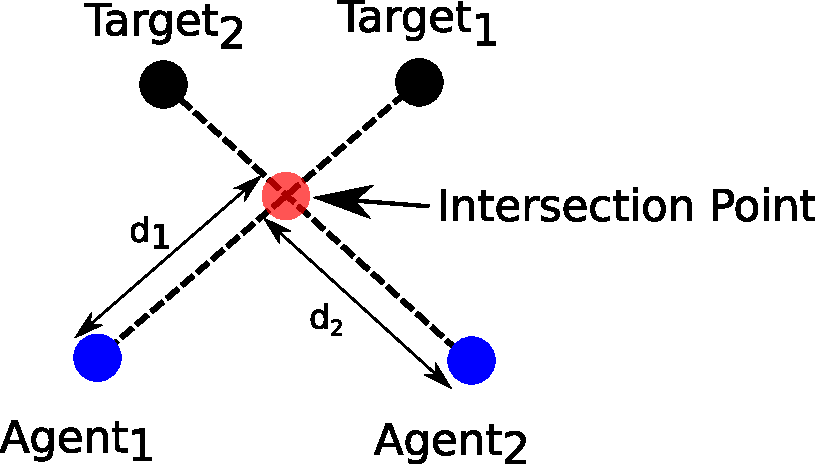
\includegraphics[width=0.6\textwidth]{Chapter4/figures/AvoidCollision.pdf}
  \caption{Collision Detection Feature in the Evaluation Function.} 
  \label{fig:AvoidCollision}
\end{figure}

Despite the exhaustive enumeration, the number of possible mappings remains small enough to find the best one in real-time. Given that the maximum number of candidate active positions in our case is 9 and the numbers of agents is 2, the number of all possible mappings is ${{9}\choose{2}}2! = 72$. In general, for $n$ positions and $k$ agents, we would have to consider ${{n}\choose{k}}k! = \frac{n!}{(n-k)!}$.




\section{Team Formation Generation}
Team formation itself is not of major focus in this thesis, but serves to set up the role assignment function and the coordination of the support subset. In general, the formation of the team is determined by the position of the ball into the field. The formation is broken up into four groups and includes all players of the team. This section presents a simple for generating team formations for both the 0.6.5 and 0.6.6 versions of the \textit{rcssserver3d} soccer simulator.

\subsubsection*{9-Players Server Version (0.6.5)}



Table~\ref{TeamFormation9} shows the four groups of roles in our formation for the 9-player team, the corresponding short identifier, and a short description for each role. 
Figure~\ref{fig:Formation9_0} shows how the different role positions of the formation are depicted into the soccer pitch. Since the formation is a function of the ball position, when the ball is located near or outside the field limits formation positions are adjusted to not exceed the field limits.



The Forwards are positioned so that they are ready for an attack at all times. If the ball is on the opponent's half of the field, Forwards are assigned positions near the ball. In particular, the Forward Center is given a position close to the ball and the other two Forwards are given positions on either side of the ball in an angle and a distance offset which are dynamically determined by the exact coordinates of the ball. If the ball is located in our half of the field, then the Forwards are given positions near the ball as in the previous case, however their positions cannot be below a limiting $X$-axis coordinate which is close to the middle of the field. 



On the other hand, Defenders are mainly positioned to guard our goal. To determine their position on the field a line segment is computed between our team's goal and the ball. The Defender Center is given a position on this line segment at a distance that ranges between 2 and 3 meters from our goal proportional to the length of this segment. The positions of the other two Defenders are located on either side of the Defender Center. 

The Midfielders are positioned to support either the Forwards or the Deferenders. When the ball is located in the opponent's half of the pitch, Midfielders are given positions near the Forwards in order to support a possible attack. When the ball is located in our half of the pitch, they are given positions in front of our defense line defined by the three Defenders.  

Finally, the Goalkeeper position is determined independently to always be in the best position to stop a shot towards our goal. 

\begin{table}[t!]
\caption{Team Formation Description for the 9-Players Version}
\label{TeamFormation9}
\begin{center}
    \begin{tabular}{cccc}
    \textbf{Group} 	 & \textbf{Role} & \textbf{Description}  \\
    \midrule
	Goalkeeper 		     & GK		& Goalkeeper  \\ 
    Defenders				& DR		& Defender Right			\\
     						& DL		& Defender Left		 	\\
    						& DC		& Defender Center			\\
    Midfielders 		    & MR		& Midfielder Right			\\
     						& ML		& Midfielder Left			\\
    Forwards  	    		& FR		& Forward Right		 	\\
     					& FL		& Forward Left		 	\\
     						& FC   	    & Forward Center		 
    \end{tabular}
\end{center}
\vspace*{-0.4cm}
\end{table}
~
\begin{figure}[t!]
\centering
  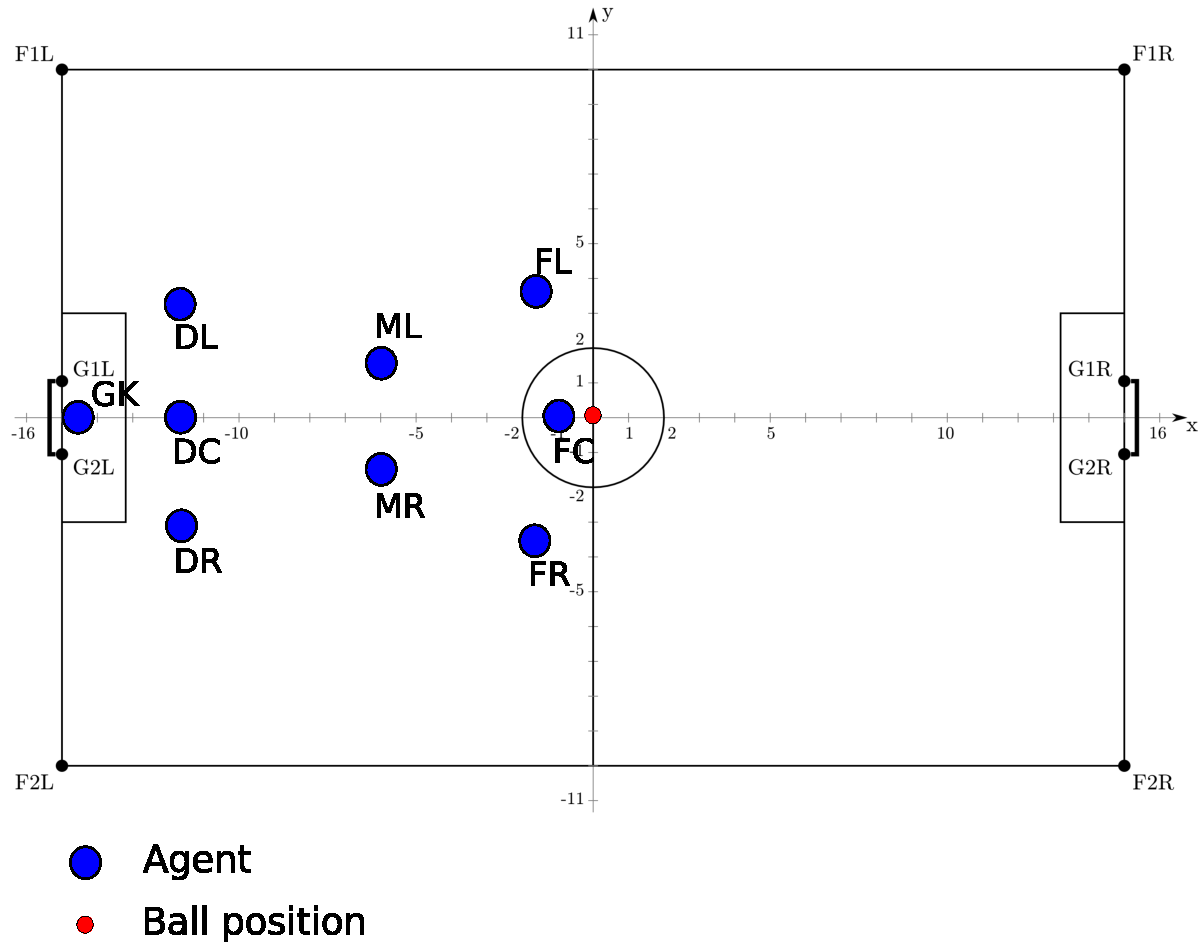
\includegraphics[width=0.7\textwidth]{Chapter4/figures/Formation9_0.pdf}
  \caption{Template of Role Positions in the Team Formation for the 9-Players Version.} 
  \label{fig:Formation9_0}
\end{figure}

\begin{table}[t!]
\vspace*{-0.5cm}
\caption{Team Formation Description for the 11-Players Version}
\label{TeamFormation11}
\begin{center}
    \begin{tabular}{ccc}
    \textbf{Group} 	& \textbf{Role} & \textbf{Description}  \\
    \midrule
	Goalkeeper 		     & GK		& Goalkeeper  \\ 
    Defenders			& DR		& Defender Right			\\
     						& DL		& Defender Left		 	\\
    						& DC		& Defender Center			\\
    Midfielders			    & MR		& Midfielder Right			\\
     						& ML		& Midfielder Left			\\
     						& MC		& Midfielder Center			\\
    Forwards 	  	  	& SF		& Forward Support         \\
     						& FR		& Forward Right		 	\\
     					& FL		& Forward Left		 	\\
     					& FC   	    & Forward Center		 
    \end{tabular}
\end{center}
\vspace*{-0.9cm}
\end{table}
~
\begin{figure}[t!]
\centering
  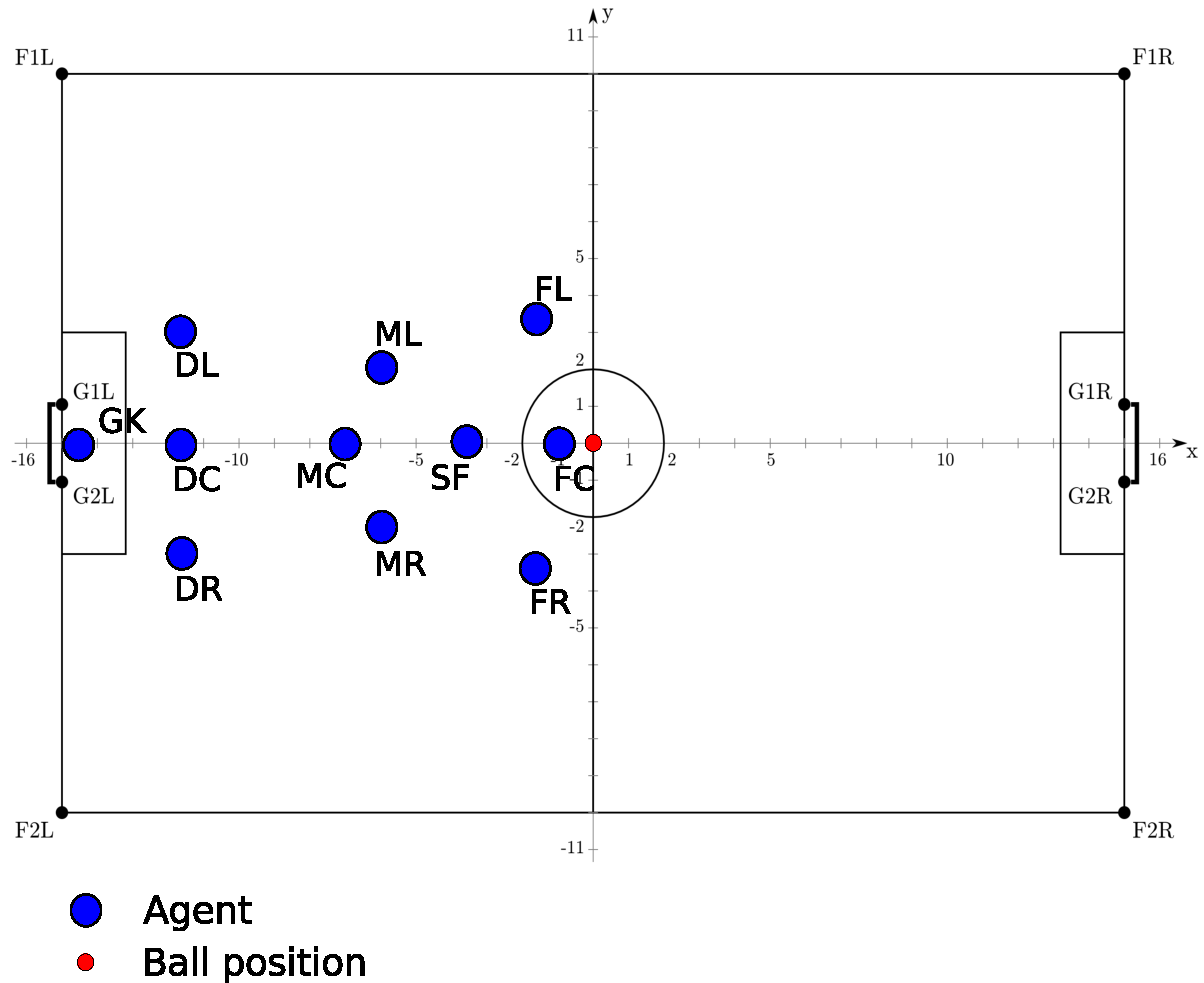
\includegraphics[width=0.7\textwidth]{Chapter4/figures/Formation11_0.pdf}
  \caption{Template of Role Positions in the Team Formation for the 11-Players Version.} 
  \label{fig:Formation11_0}
\end{figure}

\begin{figure}[t!]
\centering
  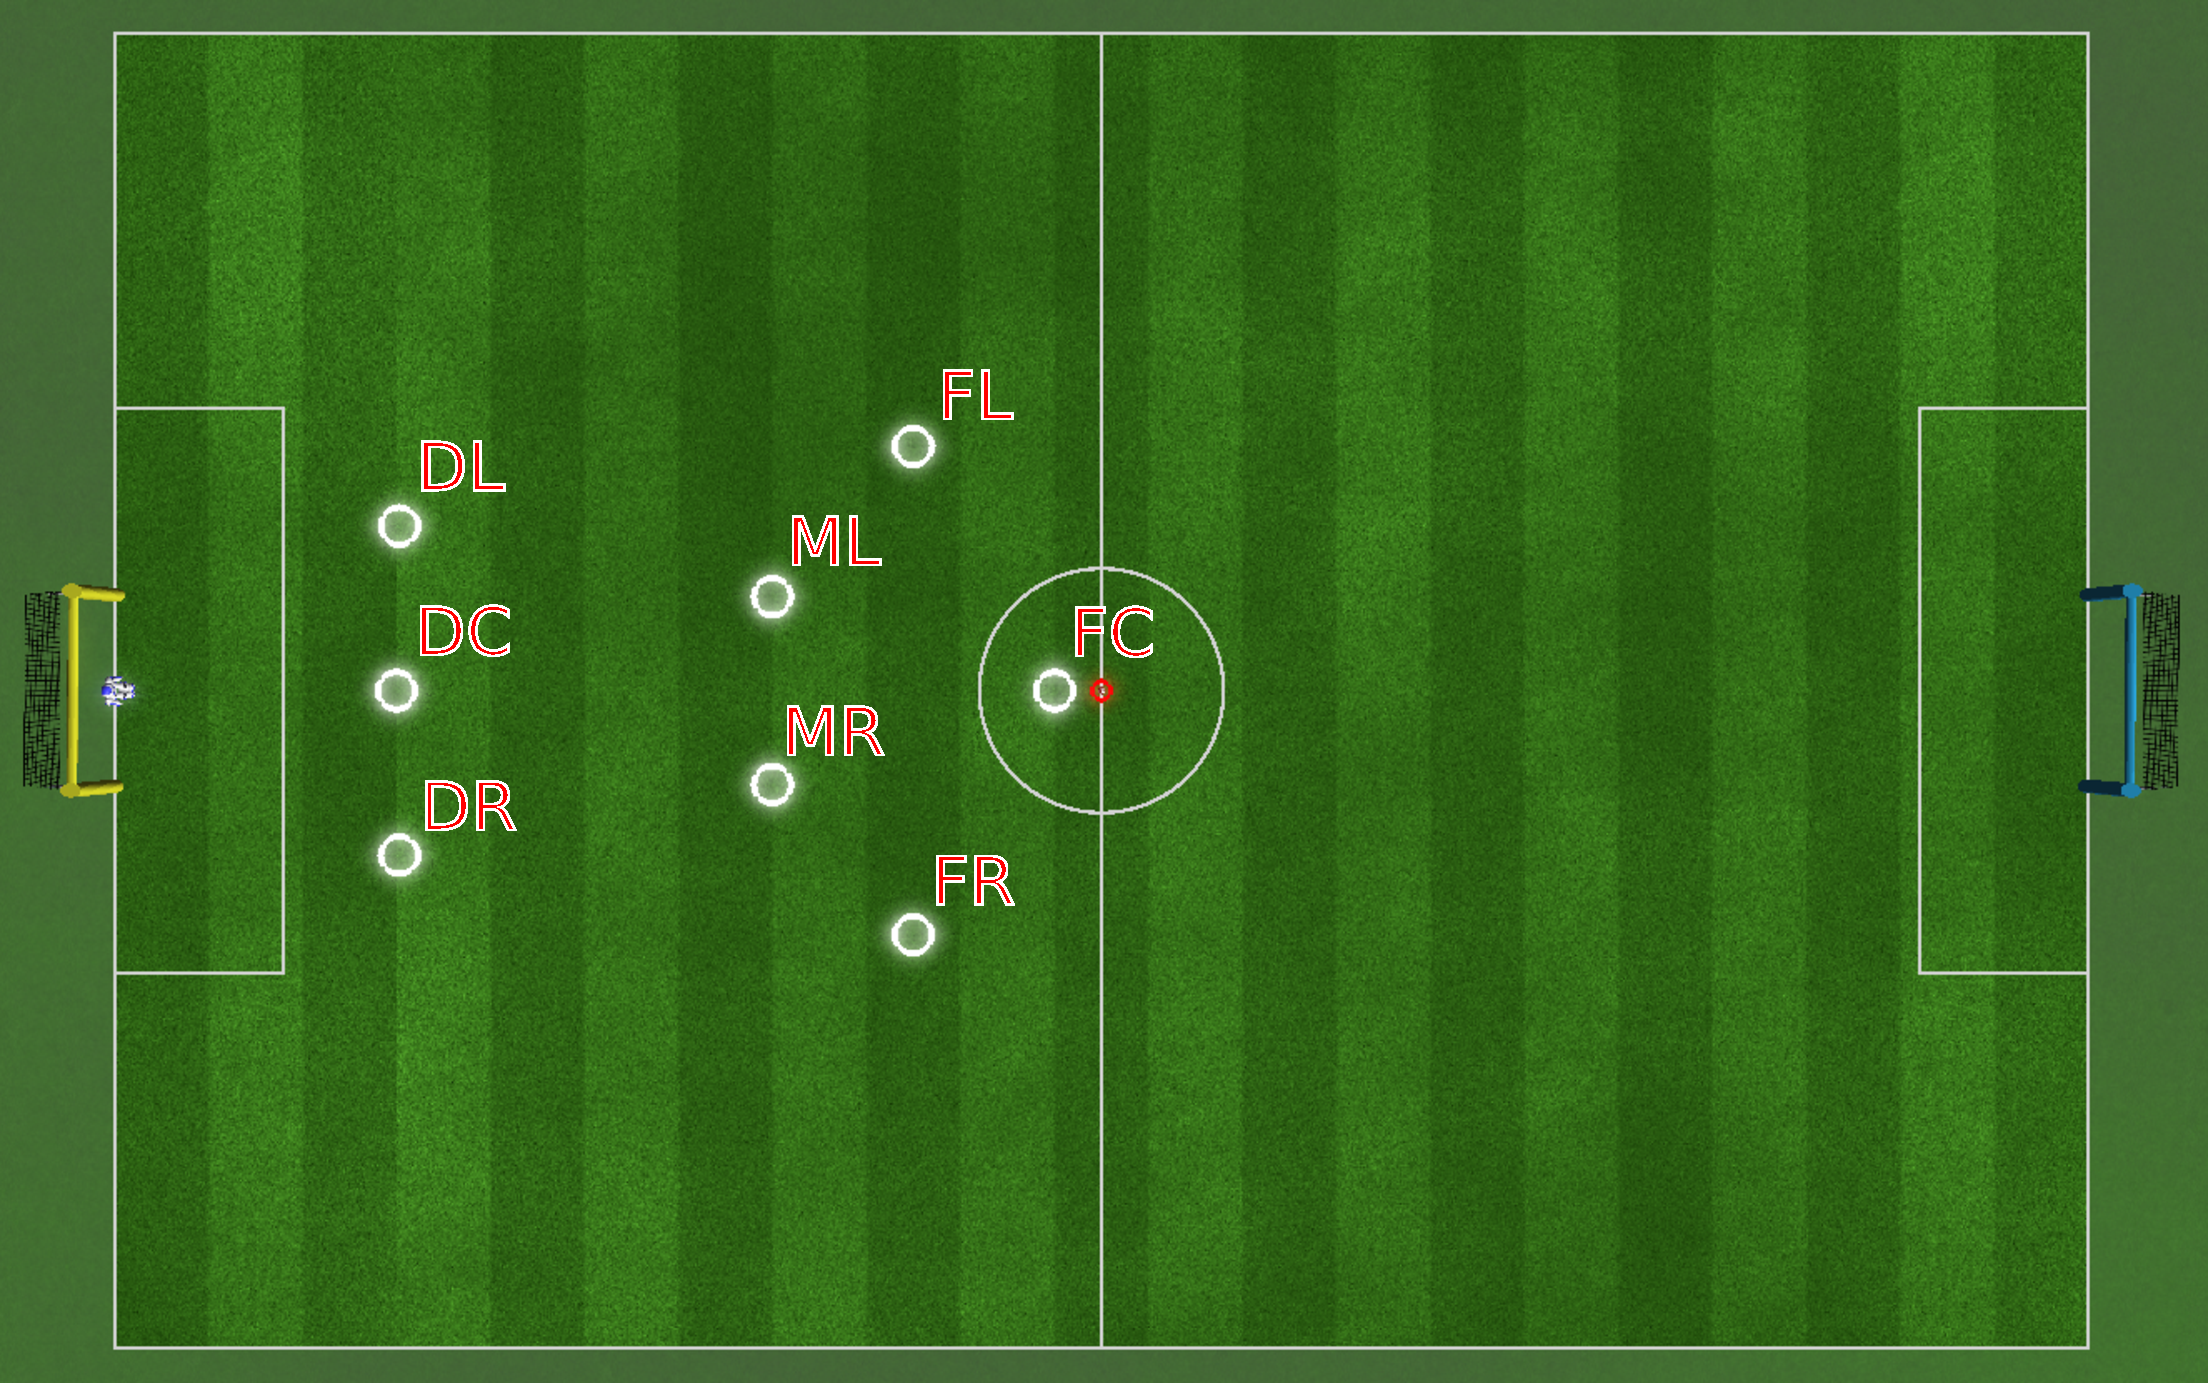
\includegraphics[height=0.3\textheight]{Chapter4/figures/Formation(0,0).pdf}\\
  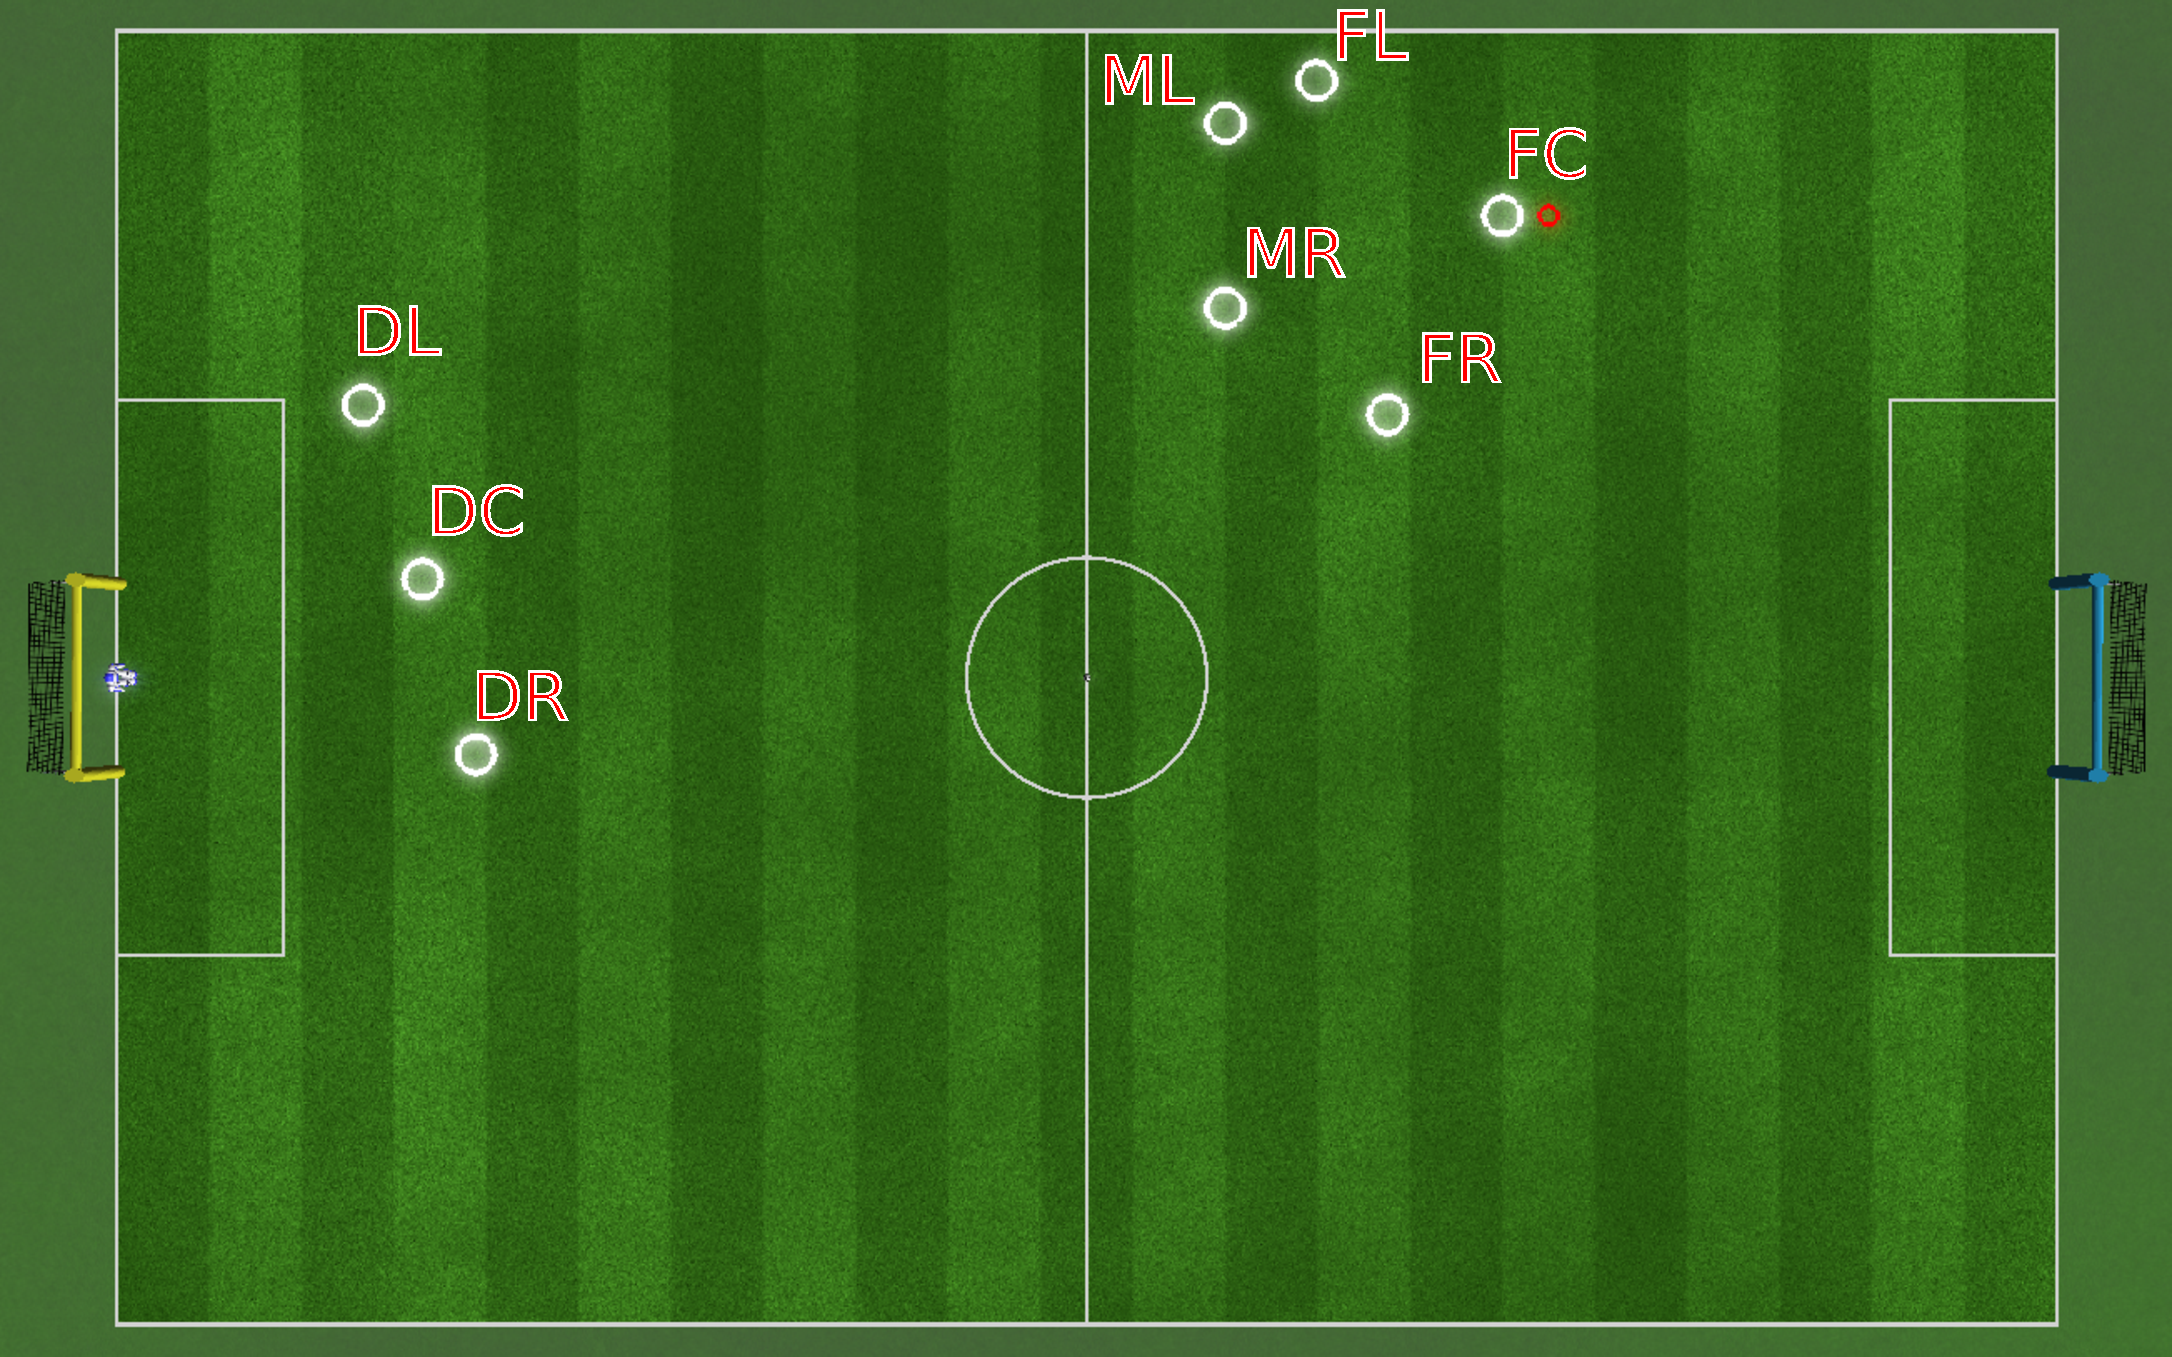
\includegraphics[height=0.3\textheight]{Chapter4/figures/Formation(5,5).pdf}\\
  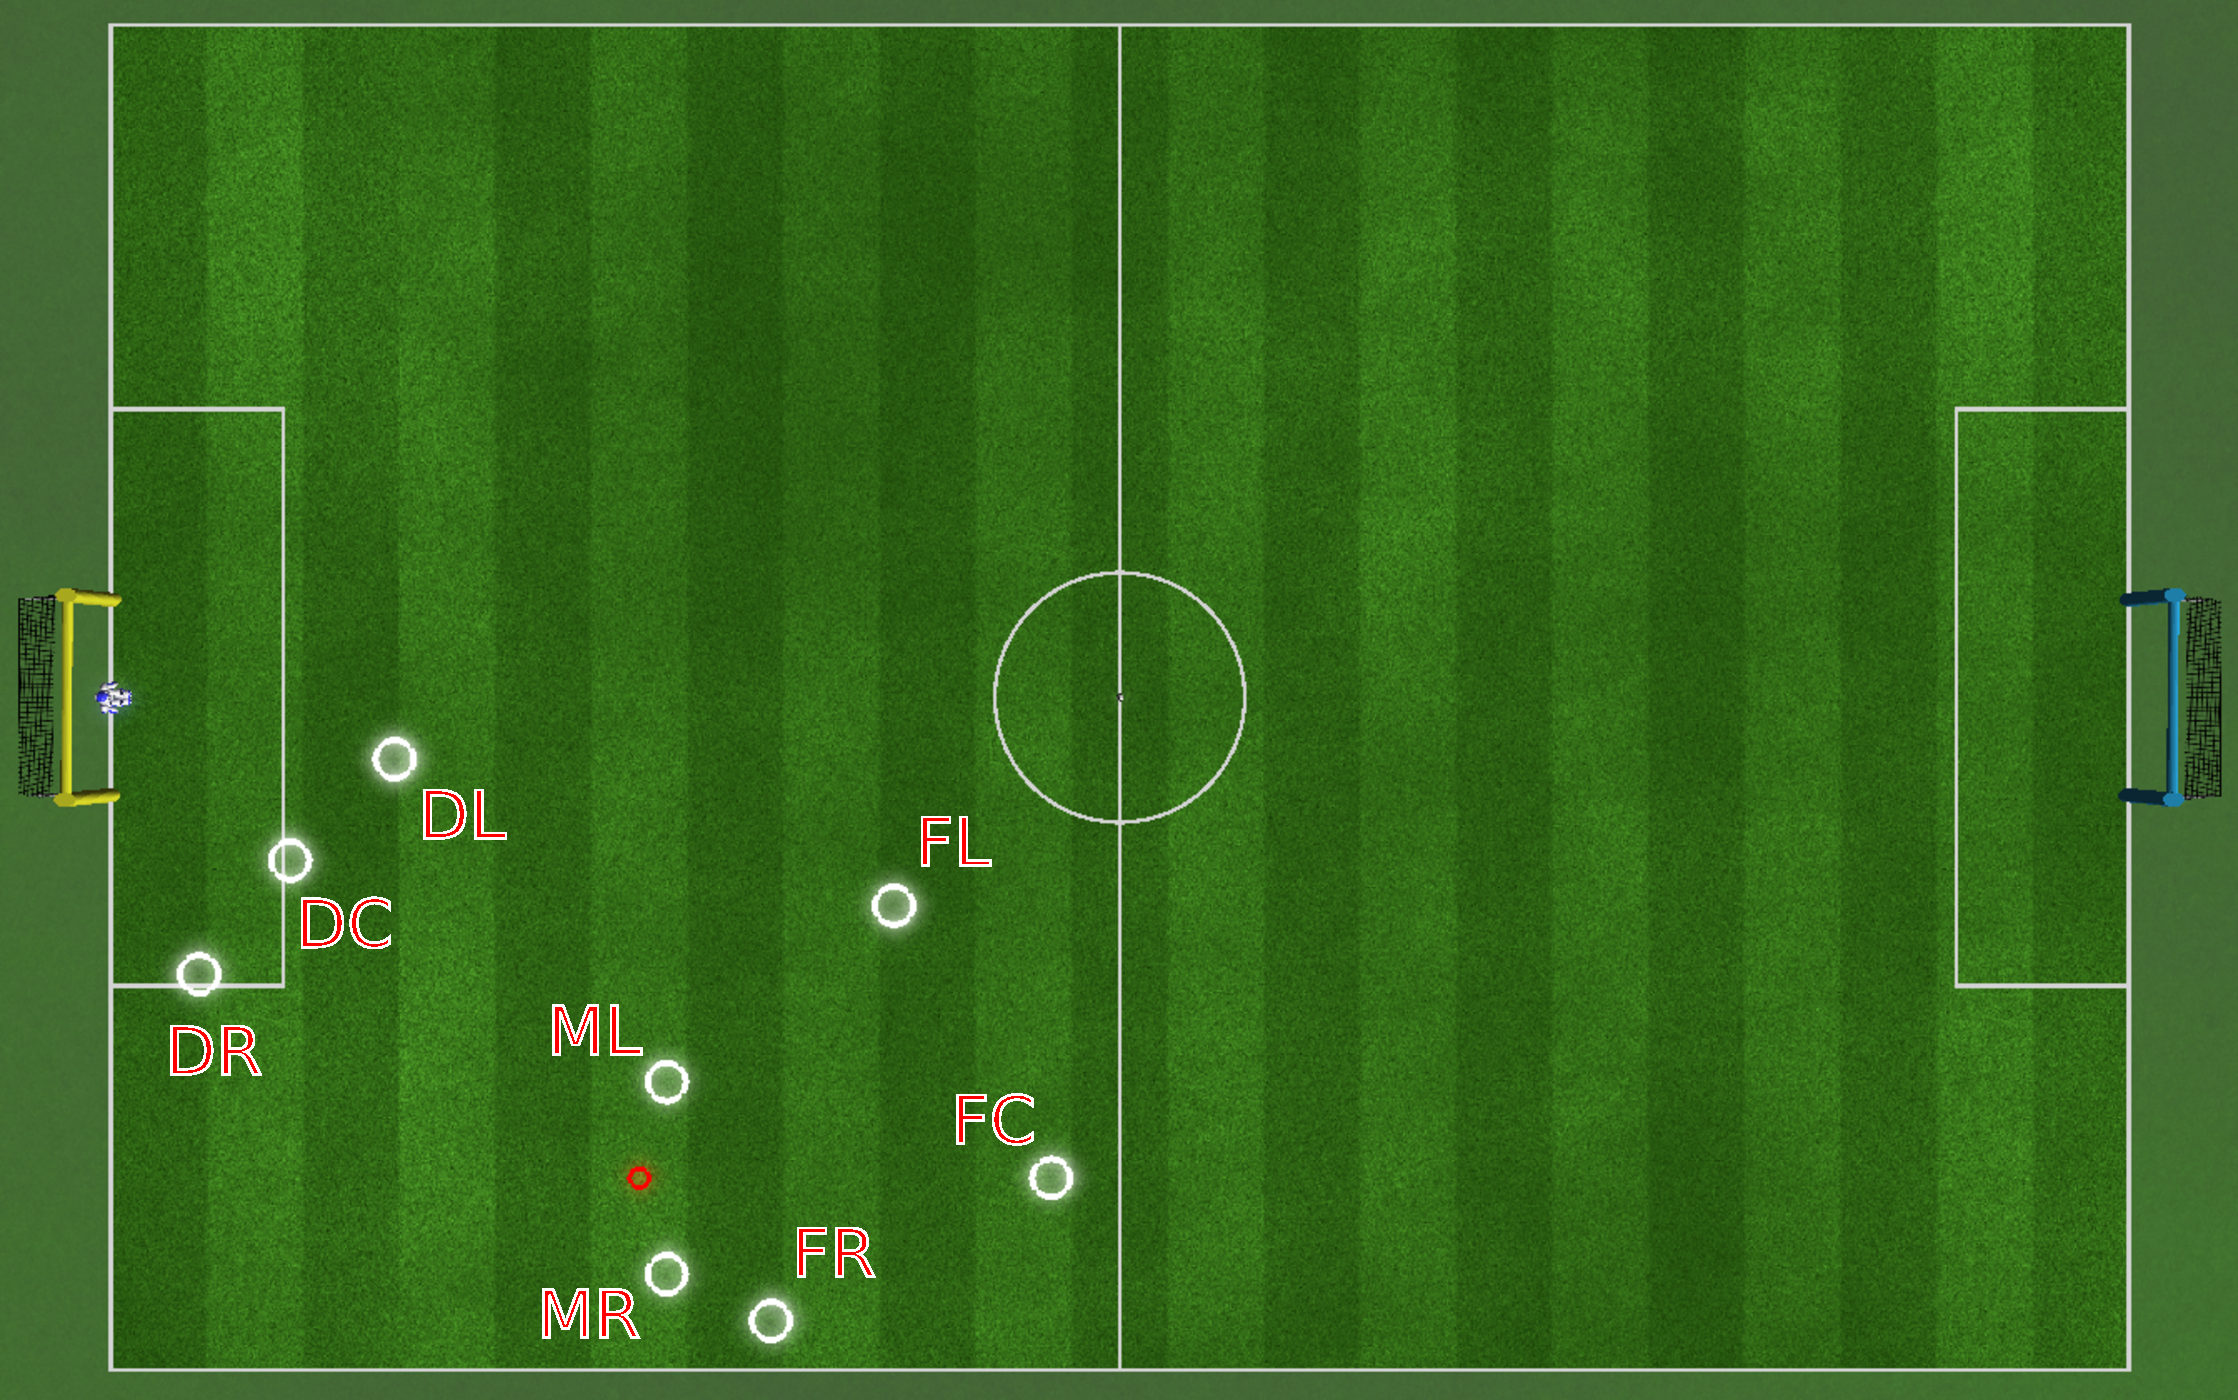
\includegraphics[height=0.3\textheight]{Chapter4/figures/Formation(-5,-5).pdf}\\
  \caption{Role Positions in Team Formation for Various Ball Positions (in red).} 
  \label{fig:FormationExamples}
\end{figure}

\subsubsection*{11-Players Server Version (0.6.6)} 

Table~\ref{TeamFormation11} shows the four groups of roles in our formation for the 11-player team, the corresponding short identifier, and a short description for each role.
Figure~\ref{fig:Formation11_0} shows how the different role positions of the formation are depicted into the soccer pitch for the newest server version in which team consists of eleven players. Again, since the formation is a function of the ball position, when the ball is located near or outside the field limits formation positions are adjusted to not exceed the field limits.


The Forwards are positioned based on the same principles as the previous version's approach. The additional player, Forward Support, is positioned behind the Forward Center at a fixed distance. The additional player in the Midfielders, Midfielder Center, is positioned behind  the Forward Support at a fixed distance. The other two Midfielder positions are on either side of the Midfielder Center in an angle and a distance offset which are dynamically determined by the exact coordinates of the Midfielder Center. The Defense line is determined exactly as in the previous version. As before, the Goalkeeper is totally independent. Figure~\ref{fig:FormationExamples} presents three different team formation corresponding to three different ball positions. 




\section{Team Roles Assignment}
In this section we present the role assignment function, which assigns roles to all agents. This will prove to be very helpful in the next coordination phase, when we have to find candidate positions for the support subset. Given a generated team formation we have to assign roles to the active subset. Recall that positions for the active agents are strictly tied to the position of the ball in the field. So, for any given number of active players, we choose an equal number of team formation positions which are closest to the ball and we assign the corresponding roles to the active players. The remaining team roles and their positions, in particular, will be available to the support subset as candidate positions during the support coordination process. Figure~\ref{fig:RoleAss} shows how the role assignment function works. Active players will be assigned the red team roles due to the fact that they are located near to the position of the ball. Note that the roles assigned to the active players will not necessarily be the three Forwards roles. Excluding the roles bound to active players, the remaining roles marked in grey are the ones the support players will compete for. A naive role mapping function would have assigned roles statically to specific players. This approach will perform poorly in such a dynamic environment. It would also be weak in situations where an agent assigned to a defensive role may end up being beamed out of field due to a penalty without being able to exchange roles with another player who may be in a better position to defend our goal. In our dynamic approach, every role mapping is calculated with a full sense of the world state, resulting in a dynamically adaptive way of assigning roles to the agents. During testing, there were several cases in which a forward player ended up assuming a defense role at the end of the game or the opposite.

\begin{figure}[t!]
\centering
  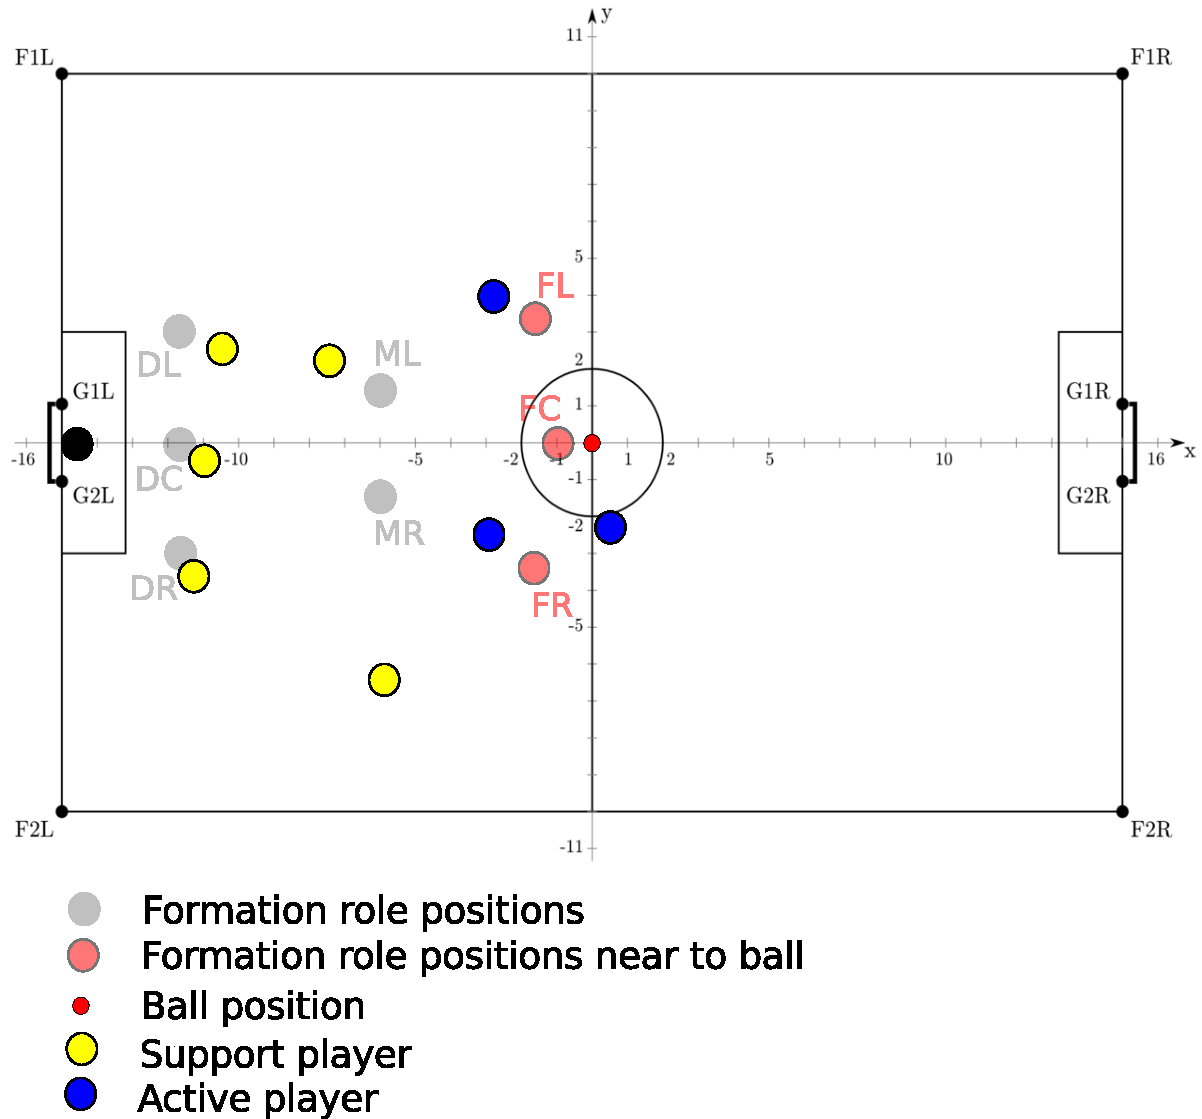
\includegraphics[width=0.8\textwidth]{Chapter4/figures/RoleAss.pdf}
  \caption{Role Assignment Function for a Given Team Formation.} 
  \label{fig:RoleAss}
\end{figure}



\section{Determination of Support Positions}
In this section, we are going to discuss about which roles and positions of the team formation will be assigned to the support subset. In an ideal case, there would be an equal number of support agents and roles/positions; this is true only when the inactive subset is empty. In this case, the positions for the support subset are determined automatically. In most cases, however, there are some inactive players and therefore we have to decide which positions of the team formation will be selected for the support subset. Using the position of the ball as a guide, we have to ensure that there will be positions for support players near the ball. So, for any given number of support players, we choose an equal number of team formation positions (excluding the ones given to the active players) which are closest to the ball and we assign the corresponding roles to the support players. Figure~\ref{fig:SupportPos} shows an example where there is one inactive player and therefore one role from the team formation is discarded, namely the one farthest away from the ball. 

\begin{figure}[t!]
\centering
  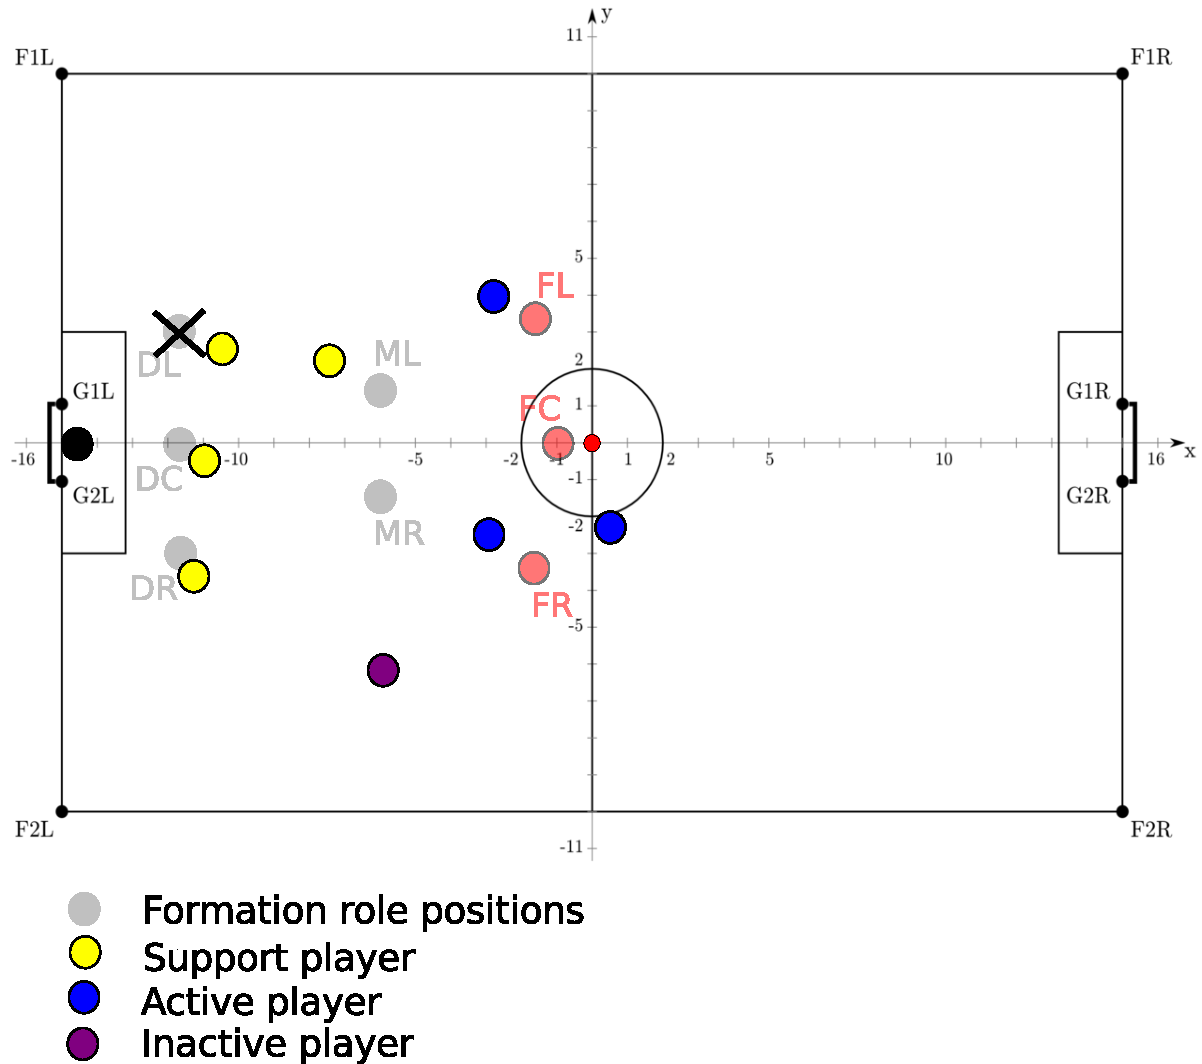
\includegraphics[width=0.8\textwidth]{Chapter4/figures/SupportPos.pdf}
  \caption{Determination of Support Positions from a Given Team Formation.} 
  \label{fig:SupportPos}
\end{figure}

\section{Support Players Coordination}
This is the final step of the coordination process, which maps support players to support positions. In Section~\ref{sec:ActiveCoordination} we showed how the active players determine such a mapping optimally. Unfortunately, this optimal algorithm is not applicable to the support subset due to prohibitive computational costs in certain cases. Given that the size of the support subset varies between 0 and 8 or 10 (depending on the server's version and the coordination type) and considering only an equal number of support positions, in the worst case the exhaustive algorithm would have to examine between 40320 and 3628800 possible mappings. Our experience has shown that the exhaustive algorithm can work satisfactorily on support subsets of size up to 6 (720 possible mappings), assuming an equal number of candidate support positions.  

Given the difficulties of applying the exhaustive algorithm to the support subset, we turned our attention to approximate, yet fast and effective, approaches in order to avoid delays in our think cycle. Our support coordination algorithm scheme is based on a method proposed by the UT Austin Villa team~\cite{UtAustinVillaPaper}. Their approach is based on dynamic programming and is able to compute an approximately optimal solution within the time constraints imposed by the duration of the think cycle ($\approx$ 20ms). Our version of this algorithm is shown as Algorithm~\ref{alg3}. Each mapping is evaluated using an evaluation function that combines some of features we used in active coordination (cf. Section~\ref{sec:ActiveCoordination}). More specifically, the evaluation function scores each possible support mapping using the Distance $C_{d,i}$ and Potential Collisions $C_{c,i}$ features defined for each agent $i$. 
The features described above are computed for each of the support agents, are weighted, and are summed to form the final evaluation function of a mapping: 
\begin{align*}
SupportCost(SupportMapping) &= \sum_{i=1}^n w_dC_{d,i}+w_cC_{c,i}
\end{align*}
where $(w_d,w_c)$ are the weights of the features, currently set at $(1,1)$. The remaining three features from active coordination are not applicable in support coordination, because the number of positions is equal to the number of agents and these features degenerate to meaningless constants. 

\begin{algorithm}[t!]
\caption{Support Players Mapping}
\label{alg3}
\begin{algorithmic}[1]
\STATE {\bf Input: }$SupportPlayers = \lbrace A_{1},A_{2},...,A_{n} \rbrace $, $SupportPositions = \lbrace P_{1},P_{2},...,P_{n} \rbrace $
\STATE {\bf Input: }$OAM=Optimal Active Mapping$
\STATE {\bf Output: }$BestSupport Mapping$
\STATE
\STATE $BestSupportMapping[s] = \emptyset$, where $s \subseteq SupportPlayers$
\STATE $BestSupportMappingCost[s] = +\infty$, where $s \subseteq SupportPlayers$
\FOR{$k = 1 \to n$} 
\FOR{{\bf each} $\alpha$ in $SupportPlayers$}
\STATE $ S = {{n-1}\choose{k-1}} $ sets of $k-1$ agents from $SupportPlayers - \lbrace \alpha \rbrace$
\FOR{{\bf each} $s$ in $S$}
\STATE $SupportMapping = \{\alpha \leftarrow P_{k}\} \cup BestSupportMapping[s]$
\STATE $SupportMappingCost = SupportCost(SupportMapping,OAM)$
\IF{$SupportMappingCost < BestSupportMappingCost[\{\alpha\} \cup s]$}
\STATE $BestSupportMapping[\{\alpha\} \cup s] = SupportMapping$
\STATE $BestSupportMappingCost[\{\alpha\} \cup s] = SupportMappingCost$
\ENDIF
\ENDFOR
\ENDFOR
\ENDFOR
\RETURN $BestSupportMapping[SupportPlayers]$
\end{algorithmic}
\end{algorithm}

 

An example of support coordination is shown in Table~\ref{tab:DynamicTable}. Mappings are built iteratively for position sets from $\lbrace P_{1} \rbrace$ to $\lbrace P_{1},P_{2},P_{3} \rbrace$ (columns from left to right) and agents sets from $\{A_1\}$ to $\{A_3\}$ and the corresponding subsets (rows from top to bottom). At each step of the algorithm, we make use of the mapping with the least cost for a subset of agents and positions (found from the previous column) which is compatible with the mapping we currently consider.


The original algorithm~\cite{UtAustinVillaPaper} is able to deliver an optimal solution due to a key recursive property, which states that in any complete mapping, if a lower cost mapping is found within some subset, then the cost of the complete mapping can be reduced by replacing the complete mapping within the subset with the lower cost mapping. This property holds for their evaluation function, which returns the maximum distance over all agents, given an assignment of positions to agents. However, this is not true for our evaluation function because of the Potential Collisions feature and therefore the best we can hope for is a good solution with no guarantees for optimality. Nevertheless, there is significant reduction in computational cost. Recall that, in the $k$th iteration of the algorithm, each agent will be assigned to the $P_{k}$ position. The previous $k-1$ positions will be assigned to the other $n-1$ agents. These assignments result in a total of $ {{n-1}\choose{k-1}} $ mappings to be evaluated in each iteration for each agent. Therefore, the total number of mappings considered for all $n$ agents and $n$ positions is:  
\[
n \sum_{k=1}^n {{n-1}\choose{k-1}} = n \sum_{k=0}^{n-1}{{n-1}\choose{k}} = n 2^{n-1}
\]
This represents a reduction to $1024$ and $5120$ mappings for $8$ and $10$ agents/positions respectively compared to $40320$ and $3628800$ mappings of the exhaustive algorithm. 



\begin{table}[t!]
\caption{Mappings Evaluated by the Support Players Mapping Algorithm.}
\label{tab:DynamicTable}
\begin{center}
\begin{small}
\begin{tabular}{ | c | c | c | }
    \hline
    $\lbrace P_{1} \rbrace$   & $\lbrace P_{1},P_{2} \rbrace$ 	& $\lbrace P_{1},P_{2},P_{3} \rbrace$\\ \hline
    $\lbrace A_{1} \leftarrow P_{1}\rbrace$ & $\lbrace A_{1} \leftarrow P_{2}\rbrace \cup \arg\min(\lbrace A_{2} \rbrace \leftarrow \lbrace P_{1}\rbrace)$	 	& $\lbrace A_{1} \leftarrow P_{3}\rbrace \cup \arg\min(\lbrace A_{2},A_{3} \rbrace \leftarrow \lbrace P_{1},P_{2} \rbrace)$  \\ 
    $\lbrace A_{2} \leftarrow P_{1}\rbrace$ & $\lbrace A_{1} \leftarrow P_{2}\rbrace \cup\arg\min(\lbrace A_{3}  \rbrace \leftarrow \lbrace  P_{1} \rbrace)$	 	& $\lbrace A_{2} \leftarrow P_{3}\rbrace \cup\arg\min(\lbrace A_{1},A_{3} \rbrace \leftarrow \lbrace P_{1},P_{2} \rbrace)$  \\ 
$\lbrace A_{3} \leftarrow P_{1}\rbrace$  & $\lbrace A_{2} \leftarrow P_{2}\rbrace \cup\arg\min(\lbrace A_{1}  \rbrace \leftarrow \lbrace  P_{1} \rbrace)$ 		& $\lbrace A_{3} \leftarrow P_{3}\rbrace \cup\arg\min(\lbrace A_{1},A_{2} \rbrace \leftarrow \lbrace P_{1},P_{2} \rbrace)$  \\ 
       						  & $\lbrace A_{2} \leftarrow P_{2}\rbrace \cup\arg\min(\lbrace A_{3}  \rbrace \leftarrow \lbrace  P_{1} \rbrace)$ 		&   \\ 
       						  & $\lbrace A_{3} \leftarrow P_{2}\rbrace \cup\arg\min(\lbrace A_{1}  \rbrace \leftarrow \lbrace  P_{1} \rbrace)$ 		&   \\ 
    						  & $\lbrace A_{3} \leftarrow P_{2}\rbrace \cup\arg\min(\lbrace A_{2}  \rbrace \leftarrow \lbrace P_{1} \rbrace)$		&   \\
    \hline
    \end{tabular}      
\end{small}
\end{center}	
\end{table}






\section{Goalkeeper Behavior}
\label{GoalKeeper}

This section presents the behavior that leads goalkeeper to make decisions and choose actions for itself. As mentioned in Section~\ref{Architecture}, the goalkeeper is the only agent in our team who ``runs'' his own behavior. His behavior depends on a finite state machine shown in Figure~\ref{fig:GoalkeeperFSM}. The initial state is the \textbf{Localize} state in which the goalkeeper tries to position himself between the two goal posts of the own goal facing the field. Once this is accomplished, the FSM switches to the \textbf{Guard} state in which it makes use of the Track Moving Object action on the ball to figure out its current position, direction, and speed. The goalkeeper stays in the \textbf{Guard} state as long as the ball is outside the goal area. If the ball moves within the goal area and there are no other agents near the ball, the goalkeeper switches to the \textbf{Libero} state in which it tries to clear the ball from the goal area while the coordination process switches to Support mode so that other players refrain from going to the ball. When the ball is cleared, the goalkeeper returns to the \textbf{Localize} state.
 
\begin{figure}[t!]
\begin{center}
\begin{tikzpicture}[->,>=stealth',shorten >=1pt,node distance=4.5cm,auto]
\node[state,initial] 		(q_1) {\textbf{Localize}};
\node[state]  			    (q_2) [right of = q_1] {\textbf{Guard}};
\node[state] 				(q_3) [right of = q_2] {\textbf{Libero}};
\draw[->] (q_1) edge [bend left=15] node {in position} (q_2);
\draw[->] (q_2) edge [bend left=30] node {ball in goal area} (q_3);
\draw[->] (q_2) edge [bend left=15] node {after fall} (q_1);
\draw[->] (q_3) edge [bend left=40] node {ball cleared} (q_1);
\end{tikzpicture}
\end{center}
\vspace*{-0.7cm}
  \caption{Finite State Machine for the Goalkeeper Behavior.}
  \label{fig:GoalkeeperFSM}
\end{figure} 
~
\begin{figure}[t!]
\centering
  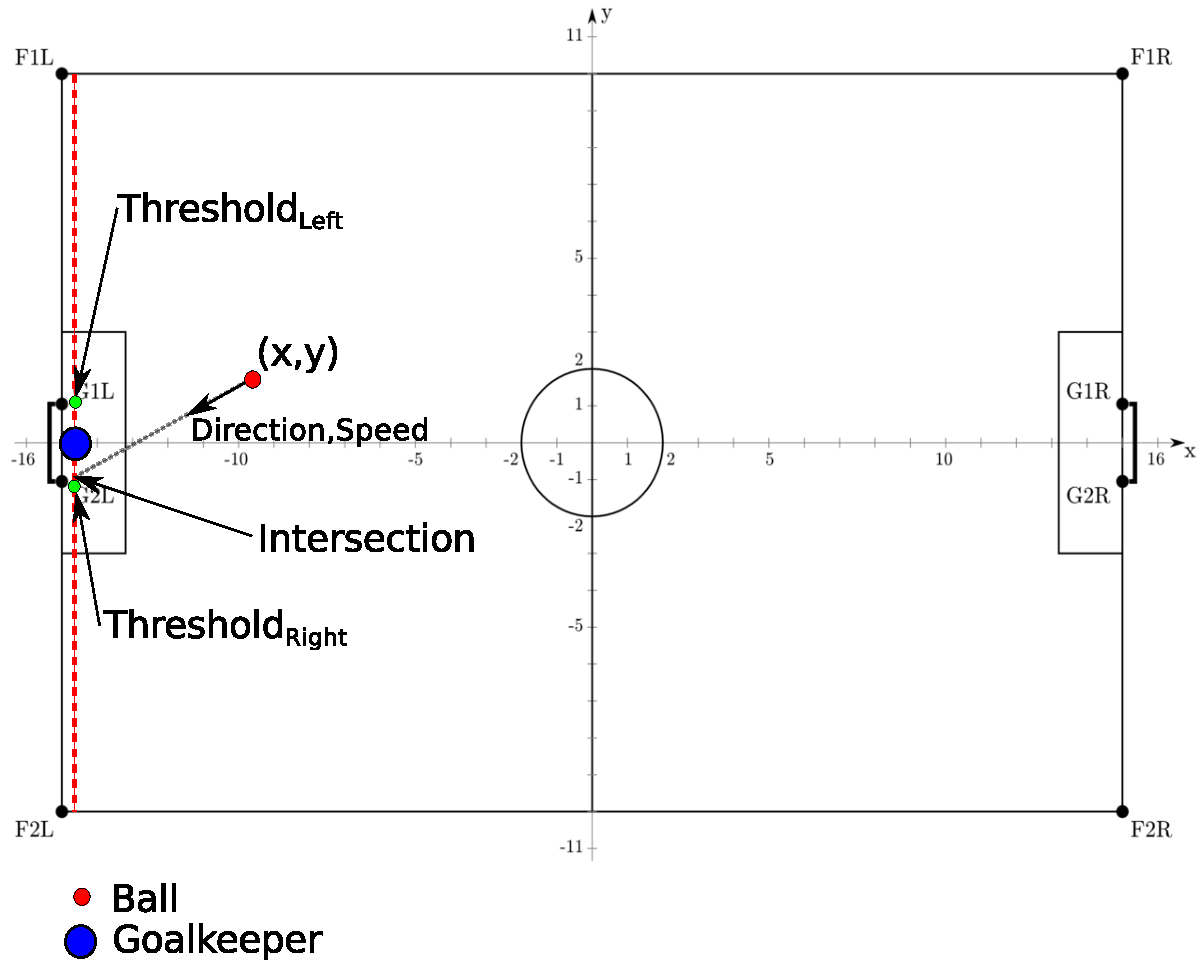
\includegraphics[trim = 0cm 0cm 10cm 0cm, clip,width=0.5\textwidth]{Chapter3/figures/Goalie.pdf}  
  \caption{Goalkeeper Behavior in the \textbf{Guard} State.}
  \label{fig:Goalkeeper}
\end{figure} 

Figure~\ref{fig:Goalkeeper} demonstrates the goalkeeper behavior in the \textbf{Guard} state. Recall that the Track Moving Object action using an egocentric reference system, marked with red dashed lines in the figure. At all times, the goalkeeper tries to compute the intersection point between its $Y$-axis and the grey dashed line which represents the direction of motion of the ball. If there is an intersection point between these two lines, the agent checks if this point falls between the two thresholds ($Threshold_{Right}$,$Threshold_{Left}$) marked in the figure. If yes, we are quite sure that the ball is heading towards our goal. We compute the time it will take for the ball to reach our $Y$-axis according to its speed and taking account the friction between the ball and the ground. If this time is less than or equal to the time it takes for our agent to fall, then the goalkeeper performs a right or left fall. An example goalkeeper fall to prevent a goal is shown in Figure~\ref{fig:GoalkeeperFall}. 

\begin{figure}[t!] 
\centering    
	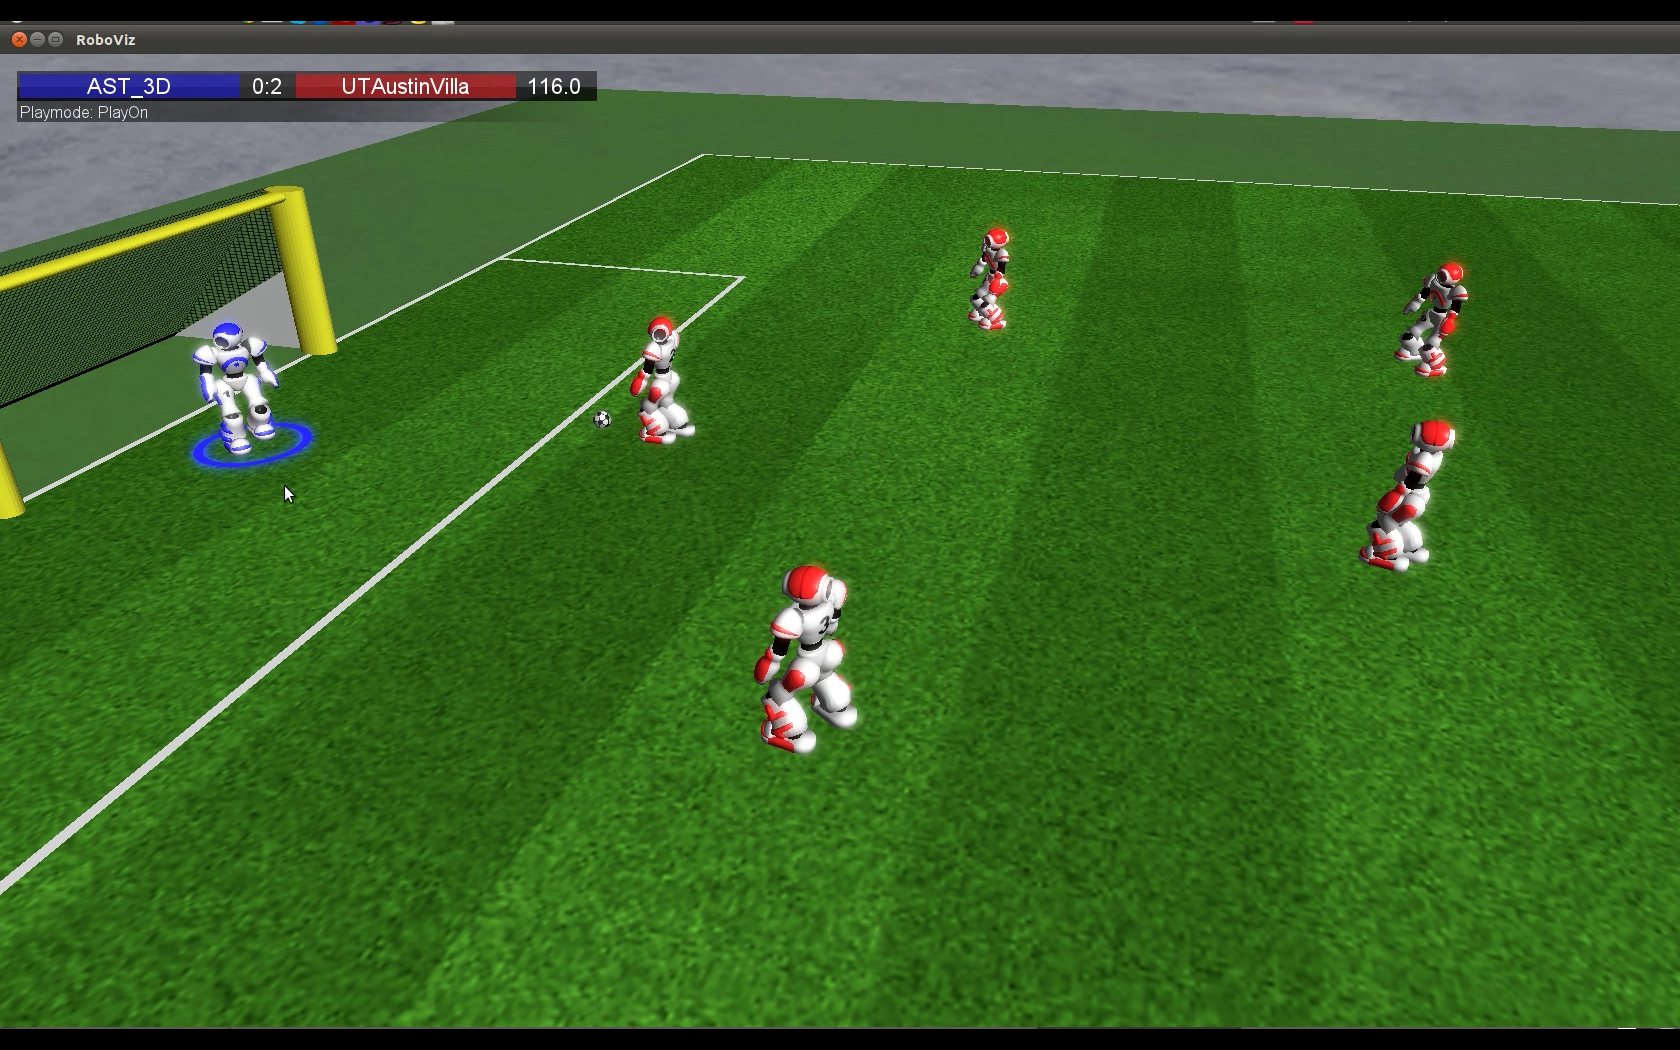
\includegraphics[trim = 5cm 10cm 30cm 5cm, clip,scale=0.25]{Chapter3/figures/GoalieFall.png}
	\quad \quad
	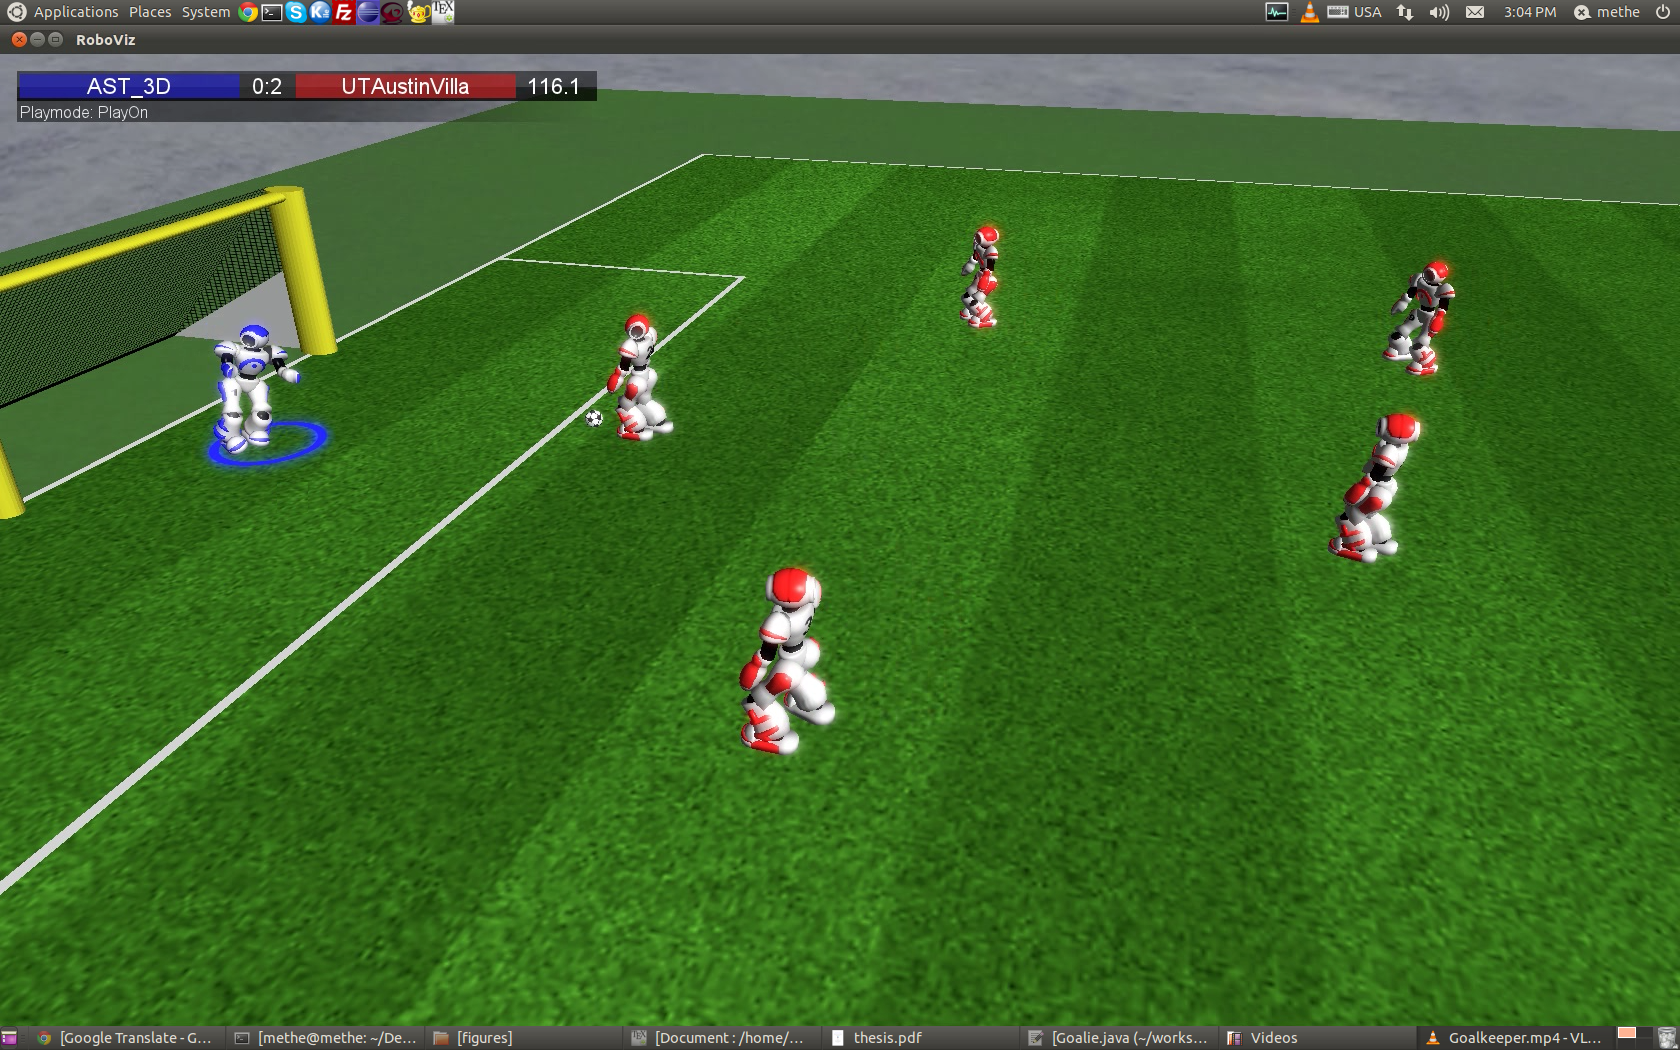
\includegraphics[trim = 5cm 10cm 30cm 5cm, clip,scale=0.25]{Chapter3/figures/GoalieFall2.png}\\
	\vspace*{1cm}
	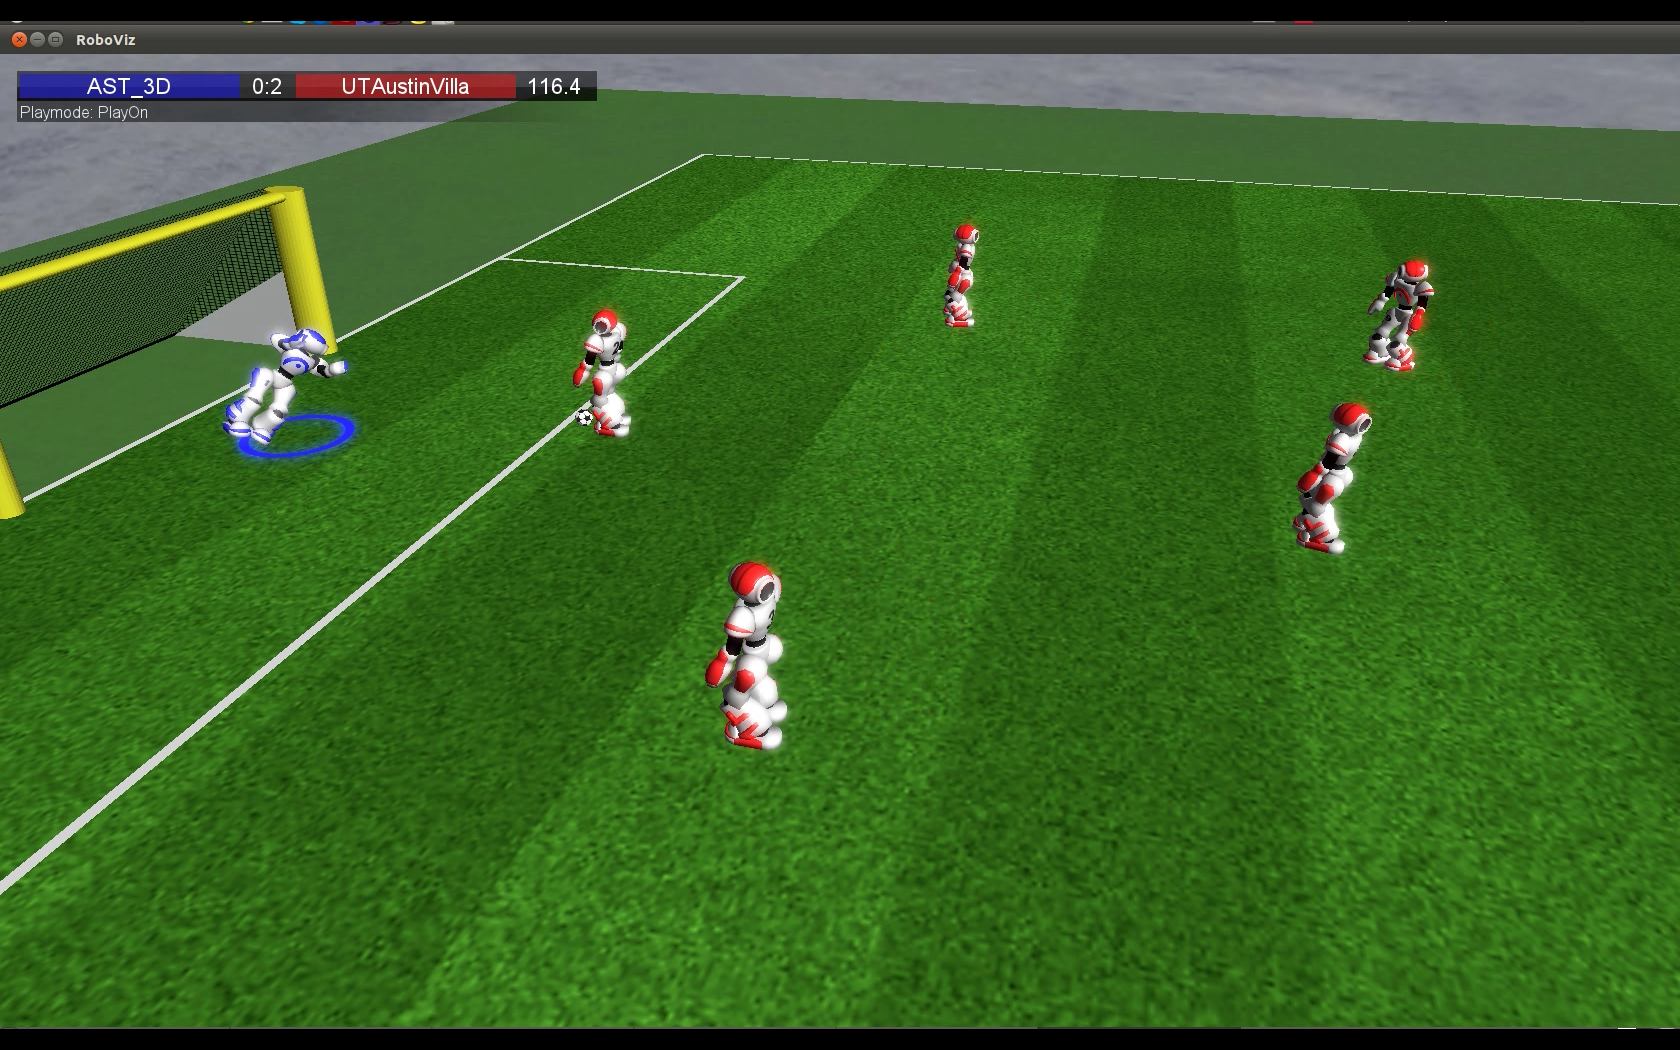
\includegraphics[trim = 5cm 10cm 30cm 5cm, clip,scale=0.25]{Chapter3/figures/GoalieFall3.png}
	\quad \quad
	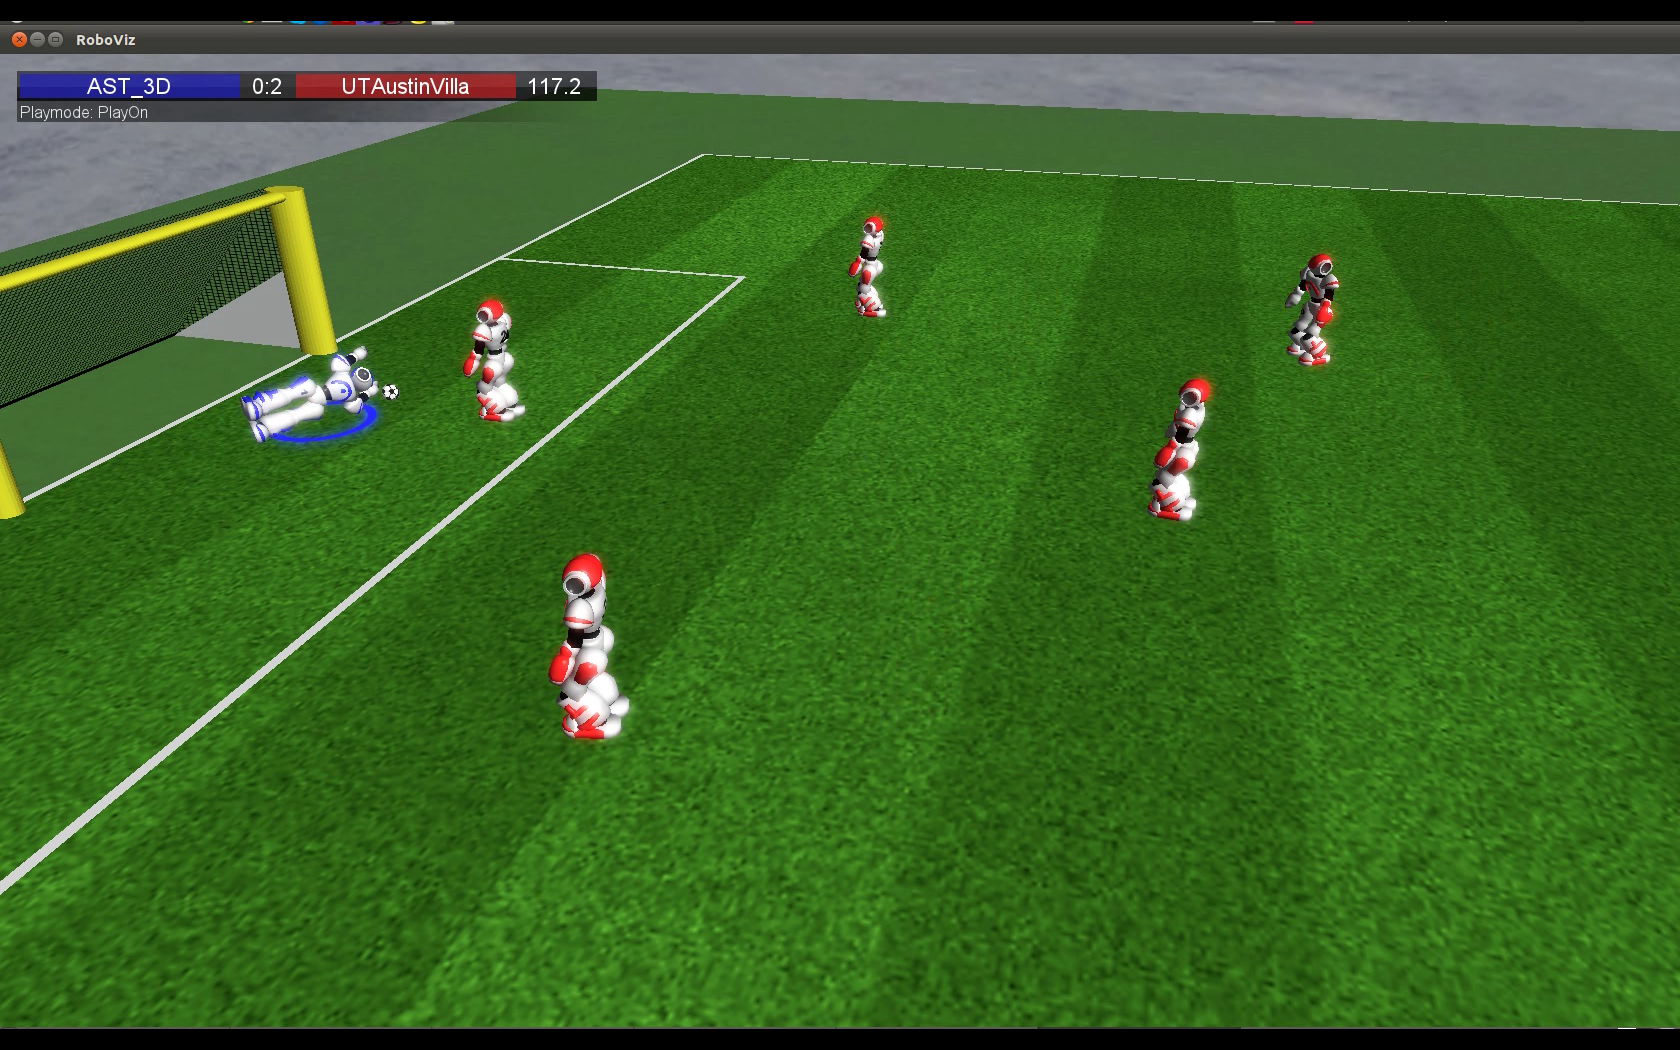
\includegraphics[trim = 5cm 10cm 30cm 5cm, clip,scale=0.25]{Chapter3/figures/GoalieFall4.png}
	\caption{An Example of a Goalkeeper Fall to Prevent Opponents from Scoring.}
  \label{fig:GoalkeeperFall}
\end{figure}